% **************************************************************************************************************
% A Classic Thesis Style
% An Homage to The Elements of Typographic Style
%
% Copyright (C) 2015 André Miede http://www.miede.de
% TUC-specific modifications in 2016 by Andreas Reinhardt 
%
% License:
% This program is free software; you can redistribute it and/or modify
% it under the terms of the GNU General Public License as published by
% the Free Software Foundation; either version 2 of the License, or
% (at your option) any later version.
%
% This program is distributed in the hope that it will be useful,
% but WITHOUT ANY WARRANTY; without even the implied warranty of
% MERCHANTABILITY or FITNESS FOR A PARTICULAR PURPOSE.  See the
% GNU General Public License for more details.
%
% **************************************************************************************************************

\RequirePackage{fix-cm} % fix some latex issues see: http://texdoc.net/texmf-dist/doc/latex/base/fixltx2e.pdf
\documentclass[ twoside,openright,titlepage,numbers=noenddot,headinclude,
                footinclude=true,cleardoublepage=empty,abstractoff, 
                BCOR=8mm,paper=a4,fontsize=11pt,11pt,a4paper,%
                ngerman,american,%
                ]{scrreprt}

%%********************************************************************
%% Get user-specific configuration
%%*******************************************************
% !TEX root = ./TUCthesis.tex

%% ****************************************************************************************************
%% 0. Set the encoding of your files. UTF-8 is the only sensible encoding nowadays. If you can't read
%% äöüßáéçèê∂åëæƒÏ€ then change the encoding setting in your editor, not the line below. If your editor
%% does not support utf8 use another editor!
%% ****************************************************************************************************
\PassOptionsToPackage{utf8}{inputenc}
\usepackage{inputenc}
\PassOptionsToPackage{T1}{fontenc} % T2A for cyrillic
\usepackage{fontenc}     


%% ****************************************************************************************************
%% 1. Configure classicthesis for your needs here. Frequently considered changes:
%% - Remove "drafting" below in order to deactivate the time-stamp on the pages
%% - Use "floatperchapter" if many floats (figures, tables, equations) exist
%% - Choose "dottedtoc" if you like page numbers to be right-aligned in the table of contents
%% For more available options see the source code of classicthesis.sty 
%% ****************************************************************************************************
\PassOptionsToPackage{	eulerchapternumbers,% use big chapter numbers in Euler math font
					listings,% add support for code listings using \lstlisting
					pdfspacing,% use pdftex for improved letter spacing
					dottedtoc,% use dotted lines in table of contents (right-align page numbers)
					floatperchapter,% enumerate tables/figures per chapter instead of consecutively
					drafting,% add version stamp at the bottom of each page
					subfig,% allow for the inclusion of subfigures in any figure environment
					beramono,% use Beramono font for monospaced text
					eulermath% use Euler math font
				     }{classicthesis}                                   
					      

%% ****************************************************************************************************
%% 2. Personal thesis-related data to auto-generate title page etc
%% Make sure to terminate each of these fields with \xspace for proper formatting
%% ****************************************************************************************************
\newcommand{\myTitle}{Extremely Long and Complicated Title of an Excellent Thesis Paper (written in \LaTeX)\xspace}
\newcommand{\myName}{Aditya Raj\xspace}
\newcommand{\myID}{123456\xspace}
\newcommand{\myThesisType}{ITIS Resarch Project Report\xspace}
\newcommand{\mySubmitDate}{15 April 2017\xspace} % format your date according to your thesis language!
\newcommand{\myThesisNumber}{ES-P005\xspace} % ask supervisor for this number - do not leave at 000!

\newcommand{\myProf}{Dr.-Ing.~Andreas Reinhardt\xspace} % Advisor and first referee
\newcommand{\myOtherProf}{Prof.~Dr.~Sven Hartmann\xspace} % Second referee
\newcommand{\myDepartment}{Embedded Systems\xspace} % Group within the Department of Informatics
\newcommand{\myLocation}{Clausthal-Zellerfeld\xspace} % Location where you will sign the statutory declaration
\newcommand{\myUni}{Technische Universit\"at Clausthal\xspace}


%% ****************************************************************************************************
%% 3. TU Clausthal specifics
%% Note that TUC only specifies four colors (one of which is a very light gray, thus unusable)
%% If you need to color text, either use \textcolor{TUDred}{text to color}
%% Alternatively, if the color shall be applied to links, specify it in the hyperref config below
%% ****************************************************************************************************
\usepackage[dvipsnames]{xcolor} % allow for TUC colors
  \definecolor{TUCgreen}{rgb}{0,0.55,0.31}
  \definecolor{TUCgrey1}{rgb}{0.5,0.5,0.5}
  \definecolor{TUCgrey2}{rgb}{0.9,0.9,0.9}
  \definecolor{TUCred}{rgb}{0.55,0.11,0}
\usepackage{tikz} % allow us to place the TUC logo on front page
\usepackage{translations} % allow us to automatically use english front matter

\usepackage{epstopdf} % for the TUC logo on the front page, when using pdflatex on Windows
\epstopdfsetup{update}

%% uncomment one of the following options if your thesis must be typeset in sans-serif font
%\usepackage[default,osfigures]{opensans}% use a sans-serif font
%\usepackage[sfdefault]{FiraSans}% use a sans-serif font


%% ****************************************************************************************************
%% 4. Loading some handy packages
%% ****************************************************************************************************
\PassOptionsToPackage{ngerman,american}{babel}   % add language support
\usepackage{babel}%	allow for proper hyphenation in languages defined above
\usepackage{csquotes}%	set quotation marks according to used language

\PassOptionsToPackage{%	add bibliography support
	backend=bibtex8,%		use BibTeX (change to biber if you know what you are doing)
	bibencoding=ascii,%		assume that BibTeX file is saved as ASCII
	language=auto,%		use hyphenation={} field in BibTeX to apply correct hyphenation
	style=numeric-comp,%	use numeric format & compress 1,2,3 to 1-3 (alternatives: numeric,alphabetic)
	sorting=nyt,% 			sorting by name, year, title
	maxbibnames=10, %	how many authors are listed before adding "et al."?
	%backref=true,%			show on which page a reference has been cited
}{biblatex}
\usepackage{biblatex}

%% math environments and more by the American Mathematics Society 
\PassOptionsToPackage{fleqn}{amsmath}
\usepackage{amsmath}

%% allow the use of acronyms (that automatically show up in the list of acronyms)
%% define any acronyms in FrontBackmatter/Contents.tex
%% Then use the acronyms in the text as follow:
%% - \ac{UML}		full spelled-out on first use, subsequently abbreviated
%% - \acp{UML}	plural case of the aforementioned one
%% - \acf{UML}	full spelled-out version, even if used before
\PassOptionsToPackage{printonlyused,smaller}{acronym} 
\usepackage{acronym} % nice macros for handling all acronyms in the thesis

\usepackage{textcomp} % fix warning with missing font shapes
\usepackage{scrhack} % fix warnings when using KOMA with listings package          
\usepackage{xspace} % to get the spacing after macros right  
\usepackage{mparhack} % get marginpar right
\usepackage{fixltx2e} % fixes some LaTeX stuff --> since 2015 in the LaTeX kernel (see below)
\usepackage{lipsum} % generate dummy text to see layout

%% ****************************************************************************************************
%% 5. Setup floats: tables, (sub)figures, and captions
%% ****************************************************************************************************

%% define how floats should be aligned. Make sure to use this in any float you add!
\newcommand{\myfloatalign}{\centering}

%% better tables. Make sure to use \tableheadline{TEXT} in each field of the headline row.
\usepackage{tabularx}
\setlength{\extrarowheight}{3pt} % increase table row height
\newcommand{\tableheadline}[1]{\multicolumn{1}{c}{\spacedlowsmallcaps{#1}}}

%% formatting for float captions (smaller font size)
\usepackage{caption}
\captionsetup{font=small}
\usepackage{subfig}  


%% ****************************************************************************************************
%% 6. Prepare code listings to use monospaced font and coloring
%% ****************************************************************************************************
\usepackage{listings} 
\lstset{language=[LaTeX]Tex,%C++,
    morekeywords={PassOptionsToPackage,selectlanguage},
    basicstyle=\small\ttfamily,% code formatting
    stringstyle=\rmfamily,% comment formatting
    keywordstyle=\color{RoyalBlue},% color of operators
    %identifierstyle=\color{NavyBlue},% color of variables
    commentstyle=\color{TUCgrey1}\ttfamily,
    numbers=left,% set this to "left" or "none" if line numbers are needed or not
    numberstyle=\scriptsize,
    numbersep=8pt,
    showstringspaces=false,% set this to "true" or "false" if spaces shall be visualized
    breaklines=true,% break too long lines
    belowcaptionskip=.75\baselineskip
} 


%% ****************************************************************************************************
%% 7. Clickable references in PDF file and citation back-references
%% ****************************************************************************************************
\PassOptionsToPackage{pdftex,hyperfootnotes=true,pdfpagelabels}{hyperref}
\usepackage{hyperref}
\pdfcompresslevel=9
\pdfadjustspacing=1 
\PassOptionsToPackage{pdftex}{graphicx}
\usepackage{graphicx} 
 
%% Reference coloring 
\hypersetup{%
    %draft,% no hyperlinking at all (useful in b/w printouts, but no clickable references)
    colorlinks=true, linktocpage=true,%	if you want hyperlinks, use this line for colored ones - OR
    %colorlinks=false, linktocpage=false, pdfborder={0 0 0},% this line for black links (e.g., for printing)
    pdfstartpage=3, pdfstartview=FitV, hypertexnames=true, pdfhighlight=/O,%
    breaklinks=true, pdfpagemode=UseNone, pageanchor=true, pdfpagemode=UseOutlines,%
    plainpages=false, bookmarksnumbered, bookmarksopen=true, bookmarksopenlevel=1,%
    urlcolor=TUCred, linkcolor=TUCgreen, citecolor=TUCgreen,%
    %urlcolor=Black, linkcolor=Black, citecolor=Black, pagecolor=Black,% any dvipscolors name can be used
    pdftitle={\myTitle},%
    pdfauthor={\textcopyright\ \myName, \myUni},%
    pdfsubject={},%
    pdfkeywords={},%
    pdfcreator={pdfLaTeX},%
    pdfproducer={LaTeX with hyperref and classicthesis}%
}   

%% Setup autoreferences
\makeatletter
\@ifpackageloaded{babel}{%
       \addto\extrasamerican{%
			\renewcommand*{\figureautorefname}{Figure}%
			\renewcommand*{\tableautorefname}{Table}%
			\renewcommand*{\partautorefname}{Part}%
			\renewcommand*{\chapterautorefname}{Chapter}%
			\renewcommand*{\sectionautorefname}{Section}%
			\renewcommand*{\subsectionautorefname}{Section}%
			\renewcommand*{\subsubsectionautorefname}{Section}%     
                }%
       \addto\extrasngerman{% 
			\renewcommand*{\paragraphautorefname}{Absatz}%
			\renewcommand*{\subparagraphautorefname}{Unterabsatz}%
			\renewcommand*{\footnoteautorefname}{Fu\"snote}%
			\renewcommand*{\FancyVerbLineautorefname}{Zeile}%
			\renewcommand*{\theoremautorefname}{Theorem}%
			\renewcommand*{\appendixautorefname}{Anhang}%
			\renewcommand*{\equationautorefname}{Gleichung}%        
			\renewcommand*{\itemautorefname}{Punkt}%
                }%  
            \providecommand{\subfigureautorefname}{\figureautorefname}%             
    }{\relax}
\makeatother


%% ********************************************************************
%% 8. Last, but not least...
%% ********************************************************************
\defbibheading{classicthesis}[\bibname]{%
  \cleardoublepage\phantomsection
  \manualmark
  \markboth{\spacedlowsmallcaps{#1}}{\spacedlowsmallcaps{#1}}%
  \addtocontents{toc}{\protect\vspace{\beforebibskip}}%
  \addcontentsline{toc}{chapter}{\tocEntry{#1}}%
  \chapter*{#1}\label{app:bibliography}%
}
\usepackage{classicthesis} 
\ifthenelse{\boolean{@drafting}}{\renewcommand{\PrelimText}{\footnotesize[draft created on \,\today\ at \thistime\xspace (\scriptsize delete \texttt{drafting} option in \texttt{thesis-config.tex} to remove this line) \footnotesize]}}{}


%% ****************************************************************************************************
%% 9. Further adjustments (talk to supervisor before changing anything below)
%% ****************************************************************************************************

\ifthenelse{\boolean{@drafting}}{
  \usepackage[textsize=footnotesize]{todonotes} % allow for inserting \todo{..} items
}{
  \usepackage[disable]{todonotes} % allow for inserting \todo{..} items
}

%% increase line spacing so your supervisor can add remarks more easily
%\linespread{1.5} 

%% add this if paragraphs should not be indented (should never be the case, though)
%\parindent0pt 

\let\marginpar\oldmarginpar %revert classicthesis change to make todonotes work
\addtolength{\marginparwidth}{10mm} % make more space for todo notes
\addtolength{\textheight}{-12mm}\addtolength{\topmargin}{14mm} % increase top margin

%% DEBUG use only
%\usepackage{showframe}


%%********************************************************************
%% Define bibliography input files (BibTeX)
%%*******************************************************
\addbibresource{Bibliography.bib}

%%********************************************************************
%% Hyphenation
%%*******************************************************
\hyphenation{Rein-hardt an-aly-sis}

%% ********************************************************************
%% GO!GO!GO! MOVE IT!
%%*******************************************************
\begin{document}

%% Some basic formatting 
\frenchspacing 
\raggedbottom 
\pagenumbering{roman}
\pagestyle{plain} 
\newcounter{dummy} % necessary for correct hyperlinks (to index, bib, etc.)

%% Uncomment one of the following options, according to thesis language.
%\selectlanguage{ngerman}\renewcommand*{\bibname}{Literaturverzeichnis}
\selectlanguage{american}


%%********************************************************************
%% Frontmatter
%%*******************************************************
%*******************************************************
% Titlepage
%*******************************************************
\ifcurrentbaselanguage{english}{\pdfbookmark[0]{Front page}{titlepage}}{\pdfbookmark[0]{Deckblatt}{titlepage}}
\begin{titlepage}
    % if you want the titlepage to be centered, uncomment and fine-tune the line below (KOMA classes environment)
  \begin{tikzpicture}[remember picture,overlay]
  \node[anchor=north west,inner sep=0pt] at (current page.north west) {
    
\includegraphics[width=\textwidth]{tuclogo/Logo_TUC_de_RGB.eps}
  };
  \end{tikzpicture}


   \begin{addmargin}[-1cm]{-3cm}
 
    \begin{center}
        \large  

        \hfill

        \vfill

        \begingroup
            \color{TUCgreen}\spacedallcaps{\Large \myTitle} \\[3cm]
        \endgroup

        
        \spacedallcaps{\myThesisType} \\[1cm]
        \ifcurrentbaselanguage{english}{presented by}{vorgelegt von}\\[0.9cm]
        \spacedlowsmallcaps{\myName}
        \\[3.4cm]

        \vfill

        %\mySubtitle \\ \medskip   
        \ifcurrentbaselanguage{english}{\myDepartment\ group}{Abteilung f\"ur \myDepartment} \\  
        \ifcurrentbaselanguage{english}{Department of Informatics}{Institut f\"ur Informatik} \\
        \myUni \\[2cm]

        \myThesisNumber

    \end{center}  
  \end{addmargin}       
\end{titlepage}   
\thispagestyle{empty}

\hfill

\vfill

\noindent\myName: \textit{\myTitle} %\myDegree, 
%\textcopyright\ \myTime

\bigskip

\noindent\ifcurrentbaselanguage{english}{\spacedlowsmallcaps{Student ID}}{\spacedlowsmallcaps{Matrikelnummer}} \\
\noindent\myID

\bigskip

\noindent\ifcurrentbaselanguage{english}{\spacedlowsmallcaps{Assessors}}{\spacedlowsmallcaps{Gutachter}} \\
\ifcurrentbaselanguage{english}{First assessor}{Erstgutachter}: \myProf \\
\ifcurrentbaselanguage{english}{Second assessor}{Zweitgutachter}: \myOtherProf

\bigskip

\noindent\ifcurrentbaselanguage{english}{\spacedlowsmallcaps{Submission date}}{\spacedlowsmallcaps{Tag der Einreichung}} \\
\noindent\mySubmitDate


\pagestyle{scrheadings}

\cleardoublepage%*******************************************************
% Declaration
%*******************************************************
\refstepcounter{dummy}
\ifcurrentbaselanguage{english}{\pdfbookmark[1]{Statutory Declaration}{declaration}}{\pdfbookmark[1]{Eidesstattliche Versicherung}{declaration}}
\ifcurrentbaselanguage{english}{\chapter*{Statutory Declaration}}{\chapter*{Eidesstattliche Versicherung}}

% Textvorschlag gemäß Anlage 4 der APO:
% Hiermit versichere ich, dass ich die Arbeit selbstständig verfasst und keine anderen als die angegebenen Quellen und Hilfsmittel benutzt habe und dass alle Stellen dieser Arbeit, die wörtlich oder sinngemäß aus anderen Quellen übernommen wurden, als solche kenntlich gemacht wurden und dass die Arbeit in gleicher oder ähnlicher Form noch keiner anderen Prüfungsstelle vorgelegt wurde.

% Textvorschlag A. Reinhardt
Ich erkläre hiermit, dass ich die vorliegende Arbeit selbständig verfasst und keine anderen als die angegebenen Quellen und Hilfsmittel benutzt habe.
\mbox{Alle} Stellen der Arbeit, die wörtlich oder sinngemäß aus anderen Quellen übernommen wurden, wurden als solche kenntlich gemacht.
Die Arbeit \mbox{wurde} in gleicher oder ähnlicher Form noch keiner anderen Prüfungs\-stelle vorgelegt.
\bigskip

% Textvorschlag gemäß Anlage 4 der APO:
% Des Weiteren erkläre ich, dass ich mit der öffentlichen Bereitstellung meiner Abschlussarbeit in der Instituts- und/oder Universitätsbibliothek einverstanden bin / nicht einverstanden bin (nicht Zutreffendes streichen).

% Alternativ-Vorschlag 1
% Hiermit erkl\"are ich mich zudem damit einverstanden, dass meine \myThesisType in der Instituts- und/oder der Universit\"atsbibliothek ausgelegt und zur Einsichtnahme aufbewahrt werden darf.

% Alternativ-Vorschlag 2
\noindent 
Ich erkläre mich zudem mit der öffentlichen Bereitstellung meines \myThesisType in der Instituts- und/oder Universitätsbibliothek einverstanden.

% Ggf. einzufügen - bitte mit Betreuer abstimmen
%
%\bigskip
%\noindent
%Ich bin damit einverstanden, dass meine \myThesisType mittels geeigneter Plagiatserkennungssoftware auf möglicherweise nicht als solche kenntlich gemachte übernommene Textpassagen oder sonstige Quellen hin überprüft werden darf.
%\todo{Mit Betreuer abstimmen, ob maschinelle Plagiatssuche erfolgen darf.}

\bigskip

\noindent\ifcurrentbaselanguage{english}{\textit{\myLocation, \mySubmitDate}}{\textit{\myLocation, den\ \mySubmitDate}}

\smallskip

\begin{flushright}
    \begin{tabular}{m{5cm}}
        \\ \hline
        \centering\myName \\
    \end{tabular}
\end{flushright}

\cleardoublepage%*******************************************************
% Abstract
%*******************************************************
%\renewcommand{\abstractname}{Abstract}
\pdfbookmark[1]{Abstract}{Abstract}
\begingroup
\let\clearpage\relax
\let\cleardoublepage\relax
\let\cleardoublepage\relax

\begin{otherlanguage}{american}
\chapter*{Abstract}
Short summary of the contents in English\dots 

A great guide by Kent Beck how to write good abstracts can be found at:  
\begin{center}
\url{https://plg.uwaterloo.ca/~migod/research/beckOOPSLA.html}
\end{center}
It is particularly important to only use the language that has been specified in its surrounding \texttt{otherlanguage} block to cater to proper hyphenation.

\end{otherlanguage}

\vfill

\begin{otherlanguage}{ngerman}
\pdfbookmark[1]{Zusammenfassung}{Zusammenfassung}
\chapter*{Zusammenfassung}
Hier eine kurze Zusammenfassung des Inhaltes in deutscher Sprache\dots 
Sollten Sie die Thesis auf Englisch schreiben, ist dennoch eine deutsche Zusammenfassung notwendig.
Im umgekehrten Fall kann die englische Zusammenfassung durch Auskommentieren weggelassen werden.
\end{otherlanguage}

\endgroup			

\vfill

%% Acknowledgments (Danksagung) can be left out if not needed
%\cleardoublepage%*******************************************************
% Acknowledgments
%*******************************************************
\ifcurrentbaselanguage{english}{\pdfbookmark[1]{Acknowledgments}{acknowledgments}}{\pdfbookmark[1]{Danksagung}{acknowledgments}}

\bigskip

\begingroup
\let\clearpage\relax
\let\cleardoublepage\relax
\let\cleardoublepage\relax
\ifcurrentbaselanguage{english}{\chapter*{Acknowledgments}}{\chapter*{Danksagung}}
Danke, Mutti!

\bigskip

Put your acknowledgments here.
Hier ggf.\ eine Danksagung einf\"ugen.

\bigskip



\endgroup





%% HINT: List of tables/figures/listings/acronyms can be uncommented in FrontBackmatter/Contents.tex
\cleardoublepage%*******************************************************
% Table of Contents
%*******************************************************
%\phantomsection
\refstepcounter{dummy}
\pdfbookmark[1]{\contentsname}{tableofcontents}
\setcounter{tocdepth}{2} % <-- 2 includes up to subsections in the ToC
\setcounter{secnumdepth}{3} % <-- 3 numbers up to subsubsections
\manualmark
\markboth{\spacedlowsmallcaps{\contentsname}}{\spacedlowsmallcaps{\contentsname}}
\tableofcontents 
\automark[section]{chapter}
\renewcommand{\chaptermark}[1]{\markboth{\spacedlowsmallcaps{#1}}{\spacedlowsmallcaps{#1}}}
\renewcommand{\sectionmark}[1]{\markright{\thesection\enspace\spacedlowsmallcaps{#1}}}

% All lines below have been commented out. If you feel like you really need a list of figures, 
% you can uncomment them back in. If in doubt, ask your supervisor if such a list should be present.

%%*******************************************************
%% List of Figures and of the Tables
%%*******************************************************
\cleardoublepage

\begingroup 
    \let\clearpage\relax
    \let\cleardoublepage\relax
    \let\cleardoublepage\relax
%    %*******************************************************
%    % List of Figures
%    %*******************************************************    
%    %\phantomsection 
%    \refstepcounter{dummy}
%    %\addcontentsline{toc}{chapter}{\listfigurename}
%    \pdfbookmark[1]{\listfigurename}{lof}
%    \listoffigures
%
%    \vspace{8ex}
%
%    %*******************************************************
%    % List of Tables
%    %*******************************************************
%    %\phantomsection 
%    \refstepcounter{dummy}
%    %\addcontentsline{toc}{chapter}{\listtablename}
%    \pdfbookmark[1]{\listtablename}{lot}
%    \listoftables
%        
%    \vspace{8ex}
%%   \newpage
%    
%    %*******************************************************
%    % List of Listings
%    %*******************************************************      
%      %\phantomsection 
%    \refstepcounter{dummy}
%    %\addcontentsline{toc}{chapter}{\lstlistlistingname}
%    \pdfbookmark[1]{\lstlistlistingname}{lol}
%    \lstlistoflistings 
%
%    \vspace{8ex}
%       
    %*******************************************************
    % Acronyms
    %*******************************************************
    %\phantomsection 
    \refstepcounter{dummy}
    \ifcurrentbaselanguage{english}{\pdfbookmark[1]{Acronyms}{acronyms}}{\pdfbookmark[1]{Abk\"urzungsverzeichnis}{acronyms}}
    \markboth{\ifcurrentbaselanguage{english}{\spacedlowsmallcaps{Acronyms}}{\spacedlowsmallcaps{Abk\"urzungsverzeichnis}}}%
    {\ifcurrentbaselanguage{english}{\spacedlowsmallcaps{Acronyms}}{\spacedlowsmallcaps{Abk\"urzungsverzeichnis}}}
    \ifcurrentbaselanguage{english}{\chapter*{Acronyms}}{\chapter*{Abk\"urzungsverzeichnis}}
    \begin{acronym}[UMLX]
      	\acro{DRY}{Don't Repeat Yourself}
		\acro{API}{Application Programming Interface}
		\acro{UML}{Unified Modeling Language}
		\acro{BS}{Base Station}
		\acro{WSN}{Wireless Sensor Network}
		\acro{SN}{Sensor Node}
		\acro{CTP}{Collection Tree Protocol}
		\acrodefplural{WSN}{Wireless Sensor Networks}
		\acrodefplural{SN}{Sensor Nodes}
		\acro{NFS-SIS}{Neighbor Finding Scheme for Sensor Information Systems}
		\acro{TWIST-CTP}{Two-hop Wireless Information System Over \ac*{CTP}}
		\acro{MAC}{Medium Access Acontrol}
		\acro{PC}{Processing Center}
		\acrodefplural{PC}{Processing Centers}
		\acro{CRC}{Cyclic Redundancy Check}
		\acro{AM}{Active Message}
		\acro{PRR}{Packet reception rate}
		\acro{ETX}{Expected number of transmissions}
		\acro{RSSI}{Received Signal Strength Indicator}
		\acro{LQI}{Link Quality Indicator}
		\acro{SFD}{Start Frame Delimiter}
		\acro{RTS}{Request To Send}
		\acro{CTS}{Clear To Send}
		\acro{DVR}{Distance Vector Routing}
		\acro{OLSR}{Optimal Link State Routing}
		\acro{RREQ}{Route Request}
		\acro{RREP}{Route Reply}
		\acro{DSR}{Dynamic Source Routing}
		\acro{AODV}{Ad-hoc On Demand Distance Vector Routing Protocol}
		\acro{RISC}{Reduced Instruction Set Computing}
		\acro{UDGM}{Unit Disk Graph Medium}
		\acro{TCP}{Transmission Control Protocol}
		\acro{UDP}{User Datagram Protocol}
		\acro{FIFO}{First In First Out}
    \end{acronym}                     
\endgroup
 

\ifthenelse{\boolean{@drafting}}{\listoftodos}{}

%%********************************************************************
%% Mainmatter
%%*******************************************************
\cleardoublepage\pagenumbering{arabic}\cleardoublepage

% !TEX root = ../TUCthesis.tex
%************************************************
\chapter{Introduction}\label{ch:introduction}
%************************************************

This bundle for \LaTeX\ has two goals:
\begin{enumerate}
    \item Provide students with an easy-to-use template for their
    Bachelor's or Master's (or even Ph.D.) thesis. 
    \item Provide a classic, high-quality typographic style that is
    inspired by ``\emph{The Elements of
    Typographic Style}'' \cite{bringhurst:2002}.
\end{enumerate}

\bigskip

This package supports acronyms (like \ac{UML}) which are defined in \texttt{Contents.tex}.
On the second use of the acronym (i.e., \ac{UML} again), it will be replaced by the short form.
If you deliberately need it spelled out, use \acl{UML} or \acf{UML}, respectively.

\bigskip

Starting from the second paragraph in a section/chapter, paragraphs are always indented.
You can avoid this by prefixed them with the \texttt{\textbackslash noindent} keyword.
If you want all paragraphs to be indented, configure this in \texttt{thesis-config.tex}.

\bigskip

\noindent If you like the style then its author would appreciate a postcard:
\begin{center}
 André Miede \\
 Detmolder Straße 32 \\
 31737 Rinteln \\
 Germany
\end{center}

You can itemize lists like this:
\begin{itemize}
\item \emph{For example} and \emph{that is} are prefixed and suffixed by a comma, i.e., like this. 
\item Of course this does not apply when starting a sentence. E.g., this is a valid sentence, too.
\end{itemize}

\section{Struktur der Arbeit}
Diese Arbeit ist wie folgt strukturiert.
In \autoref{ch:introduction} gibt es eine Einleitung.
In \autoref{ch:examples} eine Anleitung zu \emph{Getting started}.
Folgend in \autoref{ch:mathtest} ein paar mathematische Beispiele.
Eine Zusammenfassung mit Ausblick findet sich in \autoref{ch:conclusions}.




% !TEX root = ../TUCthesis.tex

%************************************************
\chapter{Background}\label{ch:Background}
%************************************************

A \ac{WSN} is a bunch of wireless devices connected together in a certain order to monitor physical or environmental conditions. Each of these devices is connected to one or several other sensors forming a network. Generally, every sensor node comprises of a radio transceiver (to send and receive messages), a microcontroller, sensors and a power source. The size of these devices can vary from the size of dust particle to the size of a notebook. They are constrained in memory, computational power, communication bandwidth and energy budget and are often deployed together in one of the several possible topologies including star, ring, tree or multi-hop mesh network. The propagation of data between the hops of the network can be routing or flooding. We can see a multi-hop mesh organisation of these nodes in figure \ref{fig:wsn-organisation}.

\par
In this figure, each of these devices have a sensor field in which they can communicate with the devices sharing a common sensor field space. The small circles in the figure \ref{fig:wsn-organisation} represent the \acp{SN} in multi-hop mesh network. In this topology, the data acquired by a \ac{SN} is routed to the sink with the help of the neighboring \acp{SN}. Finally when the data reaches the \ac{BS}, it is processed and further sent to an external network. These devices generally adhere to IEEE 802.15.4 Zigbee protocol (\cite{ieee:802.15.4}). This protocol is widely used for small low-powered digital radios and therefore find large number of application areas such as industrial Control and Monitoring, environmental and Health Monitoring, home Automation, entertainment and toys, security, location and asset tracking, emergency and disaster Response. Some of the features of this protocol include data rates of $250 kb/s (2.4 GHz)$ and $20/40 kb/s (868/915 MHz)$, $16$ channels in the $2.4 GHz$ ISM band, $10$ channels in the $915 MHz$ ISM band and one channel in the European $868 MHz$ band, carrier sense multiple access with a collision avoidance channel access, fully handshaked protocol for transfer reliability, extremely low duty-cycle $(< 10 ppm)$ capability, availability of beaconless operation and support for low latency devices.

\begin{figure}
    \centering
    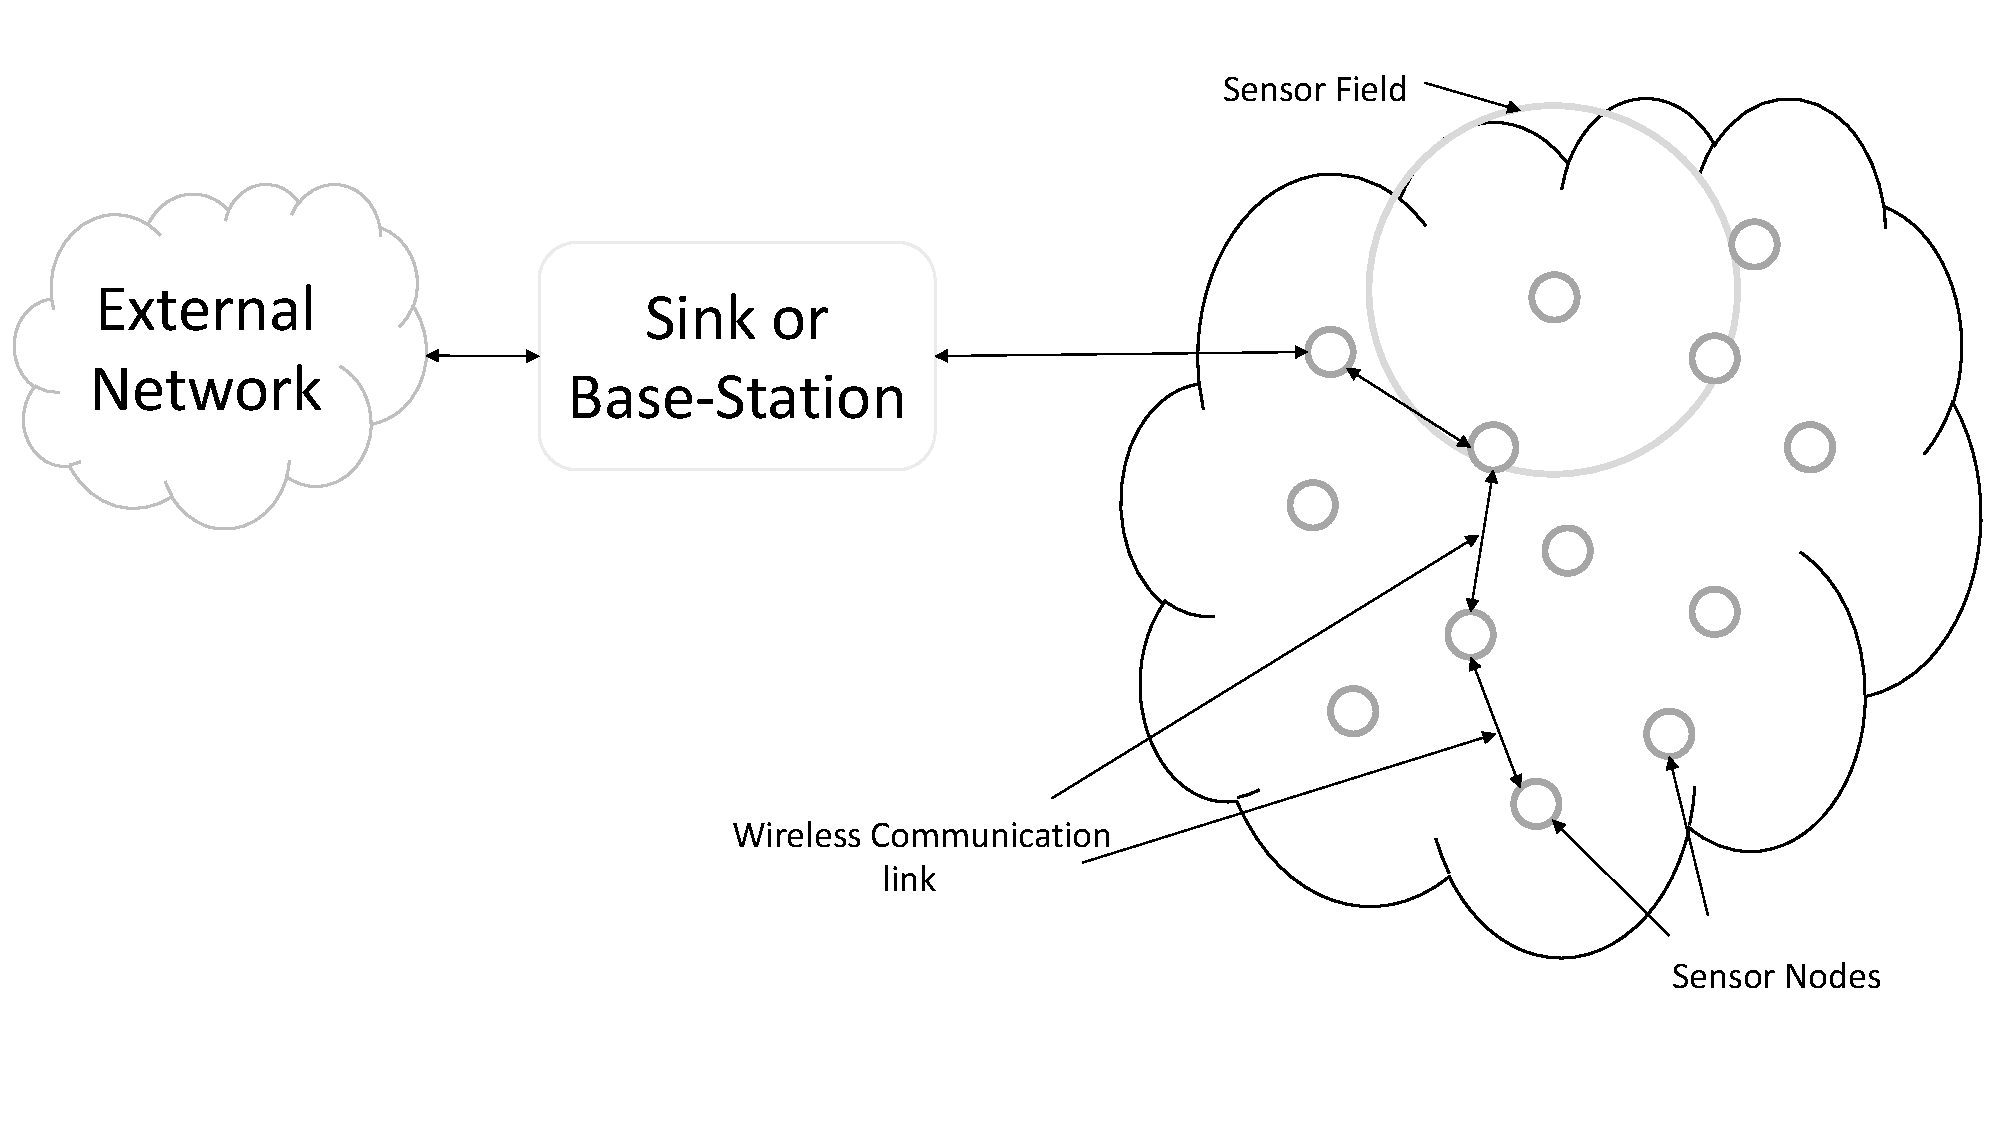
\includegraphics[width=1.0\textwidth]{gfx/WSNDiagram.pdf}
    \caption{\acp{WSN} Organisation}
    \label{fig:wsn-organisation}
\end{figure}


%************************************************
\section{Structure of Wireless Sensor Network}
%************************************************

The seven layer OSI model \cite{zimmermann1980osi}, is not suitable for implementation in low powered sensor devices. Therefore, in order to reduce the implementation complexity, the \ac{WSN} protocol stack is divided into five layers as shown in the figure \ref{fig:Wireless-Sensor-Network-Architecture}.

In this structure, each layer performs a set of tasks which is independent of other layers in the model. The physical layer deals with transferring a stream of bits over physical medium, signal detection and modulation, data encryption and connector cables compatibility with communication medium. The second layer, the data link layer provides services such as medium access control and error control, reliable data delivery, error detection and error correction. The third layer, the network layer is responsible for establishing communication paths between \acp{SN} and thereafter transmitting the packets along this path. The path selection phase depends on the one of the possible metrics: shortest path, energy efficiency, reliability and so on. The main tasks of this layer includes power conserving, partial memory, buffers, and self-organisation of \acp{SN} (because the \acp{SN} do no have universal ids). The protocols for routing layer can be separated into; flat routing and hierarchical routing or can also be separated into time driven, query-driven and event driven. The fourth layer, the transport layer provides transparent and reliable communications between end users. Two of the most widely used transport layer protocols are connection-oriented protocol, \ac{TCP} and connection-less protocol \ac{UDP}. \ac{TCP} provides reliable communication service and ensures guaranteed data delivery whereas \ac{UDP} provide an un-reliable service. In \ac{WSN} domain reliable loss recovery is more energy efficient than \ac{TCP} based communication. The final layer, the application layer is the mostly used layer for designing a\ac{WSN} application. It deals with the processing of sensed information, encryption, the formatting and storage of data and is also responsible for traffic management. It often uses information from other layers to detect if the application can meet the required resources.

\begin{figure}
    \centering
    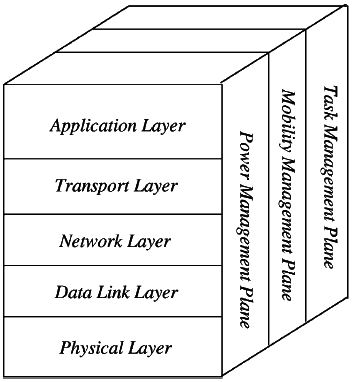
\includegraphics[width=1.0\textwidth,height=5cm]{Diagrams/Wireless-Sensor-Network-Architecture.png}
    \caption{\acp{WSN} Protocol Stack}
    \label{fig:Wireless-Sensor-Network-Architecture}
\end{figure}

\par

The three cross planes in the figure \ref{fig:Wireless-Sensor-Network-Architecture} are; power management plane, mobility management plane and task management plane. These layers help to manage the network and allow the \acp{SN} to work in conjunction with each other so that the overall efficiecy of a \ac{WSN} increases. 

%************************************************
\section{Application Areas}
%************************************************

Due to recent advancements in \acp{WSN}, it  are used in a large number of application scenarios. Some of them are listed below:

\begin{enumerate}
    \item Disaster relief operations: \acp{SN} monitor changes in environment (temperature, humidity and so on) and thus assist in disaster relief operations. They are also deployed to monitor water level in rivers to prevent flood consequences \cite{cayirci2007sendrom}.  
    
    \item Bio-diversity mapping: Observing wildlife \cite{juang2002energy}
    
    \item Intelligent buildings: Smart homes which can control the functioning of gadgets based on environmental conditions \cite{han2010smart}.
    
    \item Medicine and health care: Long-term monitoring of chronically ill patients \cite{pantelopoulos2010survey}.
    
    \item Agriculture: Monitoring soil and environment conditions to determine the amount of additives like fertilizers, water for better yield \cite{baggio2005wireless}.
\end{enumerate}

\section{nesC and TinyOS}{\label{section:nescTinyOS}}
%************************************************
This section will describe about the fundamentals of using nesC programming language (\cite{website:nesc}) in TinyOS. In the first subsection we will explain about the structure of a nesC program and in second part we will describe about the abstractions involved in sending and receiving messages using TinyOS. We will also talk about the data structures offered in TinyOS and finally we will describe the limitations of using TinyOS.   

    %************************************************
    \subsection*{nesC}
    %************************************************
    
    As an extension to C programming language, it defines the structure of TinyOS applications in components. The components are further modularized into interfaces, modules and configurations. Let us go through them one by one:
    
    \begin{enumerate}
        \item Interfaces:
        
        The notion of interface in nesC is similar to the concept of \textit{Interfaces} in Java or any other Object-oriented programming language. They define methods that can be implemented by a module. However, a major difference is: only events defined under interfaces must be implemented and commands can be called whenever required. For example Leds Interface provides these methods:
        
        \begin{lstlisting}
        
            interface Leds {
            
              // Turn on LED 0.
              async command void led0On();
            
              //Turn off LED 0.
              async command void led0Off();
            
              /**
               * Toggle LED 0; if it was off, turn it on, if was on, turn it off.
               * The color of this LED depends on the platform.
               */
            async command void led0Toggle();
            
            ...
            ...
        \end{lstlisting}
        
        Now to turn on the Leds on the Telosb, when required, we need to first use the interface called $Leds$ in our application by stating the following:
        
        \begin{lstlisting}{language = C}
            use interface{
                Leds;
            }
        \end{lstlisting}
        
        Then we have to call methods provided by Leds interface in our implementation. Leds interface provide methods to toggle(Leds.Led0toggle()) or turn on (Leds.Led0toggle()) the Leds on telosb board. Telosb led lights can be turned on by giving the command: 
        
        \begin{verbatim}
            call Leds.Led0On();
        \end{verbatim}
        
        We must note here that interfaces are prefixed with \textit{call} keyword. Also, there are parametrised interfaces to support multiple instances of same interface. The parameters for these multiple instances of interfaces can be small small integers.
        
        \item Modules and Configurations: Having discussed the interfaces concept, we will now look at the overall structure of a nesC program. A nesC program has two components: a file containing a module with its implementation, also known as \textit{Modules} and another file with configuration including the implementation, also called as \textit{Configurations}. Configurations, describe the wiring structure of components. In contrast to Configurations, Modules are implementations. Configurations connect the declarations  of  different  components,  while  modules  define  functions  and allocate state.
        
        Both modules and configurations can provide and use interfaces, but the main difference lie in their implementations. \textit{Configuration} implementations refer to how the interfaces used in modules are wired to the actual component that provides it. While \textit{Module} implementations are piece of executable codes that define how the provided interfaces should execute and return or how to use the interfaces to provide a new functionality. This will be clear in following example:
    
    \noindent\begin{minipage}{.40\textwidth}
    \begin{lstlisting}[title=Module,frame=tlrb]{Name}
    module BlinkC @safe()
    {
        uses interface Leds;
        uses interface Boot;
    }
    implementation
    {
        event void Boot.booted()
        {
            call Leds.led0Toggle();
        }
    }
    \end{lstlisting}
    \end{minipage}\hfill
    \begin{minipage}{.40\textwidth}
    \begin{lstlisting}[title=Configuration,frame=tlrb]{Name}
    configuration BlinkAppC
    {
    }
    implementation
    {
      components BlinkC, LedsC;
      BlinkC.Leds -> LedsC;
    }
    \end{lstlisting}
    \end{minipage}
    
    \end{enumerate}
    
    \par
    
    In the above code, the module section uses interface Leds and the implementation section calls \textit{Leds.led0Toggle()} to turn on the Leds on Telosb. Now, in the configuration section we need to instantiate LedsC component and further wire it to Leds interface used in module section so that the TinyOS points to the actual implementation of Leds, provided by LedsC component.

    %************************************************
    \subsection*{TinyOS}
    %************************************************
    
    TinyOS (\cite{website:TINYOS}) is the de facto standard in the field of \acp{WSN}. It provides network protocols, device driver for different sensor platforms, data capturing tools, single-hop networking, ad-hoc routing, timers and many other features, which can be easily used, with suitable modifications, for different application domains. It follows event-driven model which helps to run concurrent applications using small amount of memory. TinyOS uses Event driven models because they are faster than stack threaded design. This is because of two main reasons: 1. They do not require in-advance memory reservation to save execution context. 2. Hardware, is always split-phase rather than blocking. Because of non-blocking operations they perform the operations rapidly. In idle state, it goes in sleep state to save energy.
    
    \par
    A \ac{FIFO} based TinyOS scheduler schedules operations of components. This is also power efficient because the device can go in low power state when the queue is empty. Components are a collection of \textit{Command Handlers}, \textit{Event Handlers} and \textit{Tasks}. They contain the declarations of commands and events which are provided by the interface it uses or provides. After the declaration in Modules section, the interfaces in an application can be wired to the components which actually implements them. Let us look at these three components one by one:
    
    \begin{enumerate}
        \item Commands: Commands are non-blocking requests made to low-level components and therefore must return with the exit status whether it was successful or not. Commands can also schedule tasks for later execution. This will involve event handlers which can in turn execute other low level commands.
        
        \item Events:  In an embedded system application, we primarily focus on  handling events. In general, events are generated or triggered in response to some action that has been initiated by commands. Interfaces contain commands and events, and therefore when we use an interface, we must implement all the events, so that appropriate actions are defined when events are fired.
        
        \item Tasks: Tasks enable components to perform general-purpose "background" processing in an application. They are  non preemptive. This  means  that  only  one  task  runs  at any time, and TinyOS does not interrupt one task to run another. Once a task starts running, no other task runs until it completes. This means that  tasks  run  atomically  with  respect  to  one  another. This  has  the nice  property  that we  don’t  need  to  worry  about  tasks  interfering with one another and corrupting each other’s data. However, it also means that tasks should usually be reasonably short. If a component has a very long computation to do, it should break it up into multiple tasks. A task can post itself.
    \end{enumerate}
    
    \par
    To understand these components, we will consider the structure of AMSenderC component:
    
    \begin{verbatim}
        provides {
            interface AMSend;
            interface Packet;
            interface AMPacket;
            interface PacketAcknowledgements as Acks;
        }
    \end{verbatim}
    
    In the above example, if \textit{AMSend} interface is wired to \textit{AMSenderC} then it will be called as implemented in \textit{AMSenderC} component. Now, if we invoke \textit{AMSend.send()} method (provided by \textit{AMSend} interface) with a network packet (which is of type nx\_uint8\_t or nx\-uint16\_t) then it will schedule a task to send the packet which in turn will invoke an event handler \textit{AMSend.SendDone()} to acknowledge, if the sending operation was successful or not. Other aspects related to networking design will be covered further in \ref{subsec:network-architecture}
    
    \par
    There are following limitations in TinyOS:
    
    \begin{enumerate}
        \item Dynamic memory allocation is not allowed. This prevents run time memory allocation failures and memory fragmentation.
        
        \item Function pointers are also not allowed because TinyOS needs to know the complete execution graph of the program in advance.
    \end{enumerate}
    
    %************************************************
    \subsection*{TinyOS Networking Architecture}\label{subsec:network-architecture}
    %************************************************
    
    The maximum size of a TinyOS packet is 128 bytes including its headers and \ac{CRC}, which also matches the 802.15.4 specifications. An increase in packet size can lead to unpredicted errors in TinyOS. The core of communication abstraction comes from Active Messages (AM), a single-hop unreliable packet. They have a destination address and provide synchronous acknowledgement. The interfaces to send and receive messages in TinyOS are listed below:
    
    \begin{itemize}
        \item AMSend: This interface is used to send a message by calling the AMSend.Send command (provided by AMSend interface). On completion of successful or unsuccessful sending SendDone event is signalled. In general \ac{WSN} application development scenario, we also using this event as an indicator to send the next packet. 
        
        \item AMReceive: On reception of a message sent via AMSend interface, AMReceive.receive event of the corresponding AMSender id is signalled.
        
        \item AMSnoopingReceiver: This interface signals event AMSnoopingReceiver.receieve even when the packet is not addressed to a particular \ac{SN}. This allows us to snoop packets in the device communication range.
    \end{itemize}
    
    To send data, we need to instantiate a member of AMSend with an am\_id\_t type, which is a small integer, and further wire it to AMSend interface. We then need to call AMSend.send() method from the module implementation, which will trigger sending of \ac{AM} packet. The packet can either be sent to all the sensor nodes which is done by broadcasting at AM\_BROADCAST\_ADDR (a constant defined as 0xFFFF and is reserved in TinyOS for broadcasting purposes) or to a specified TOS\_NODE\_ID (every \ac{SN} has a specific address which can be obtained by calling TOS\_NODE\_ID constant).
    
    \par
    After a \ac{SN} receives an \ac{AM}, it calls events that are responsible to receive the messages of the defined \textit{am\_id\_t} type of Receive Component. This concept of multiple instances of same Component, gives us the flexibility to have multiple instances of Receivers (abstracted as \textit{AMReceiverC}). With multiple \ac{AM} ids of AMReceiverC, the device will only call the event associated with the matching receiver id. This concept is predominantly used in TinyOS to distinguish messages of different types and we will also use this in implementation of the concept \textit{heterogeneity} to distinguish one hop and two hop messages received. 
    
% This section describes how \ac{PC} advertises it's availability, \acp{SN} discovers the \ac{PC} and finally how data transfer takes place.

%************************************************
\section{Route Finding and Selection}    
%************************************************

Route discovery, route selection and route representation are key requirements for a wireless multi-hop routing problem. Therefore, it becomes quite important to decide appropriate protocols for finding a solution to multi-hop routing scenarios. We will cover the fundamentals to find a solution to the multi-hop routing problem by sequentially enumerating through the mentioned phases, as shown in the figure \ref{fig:RouteFinding}:

\begin{figure}[h]
    \centering
	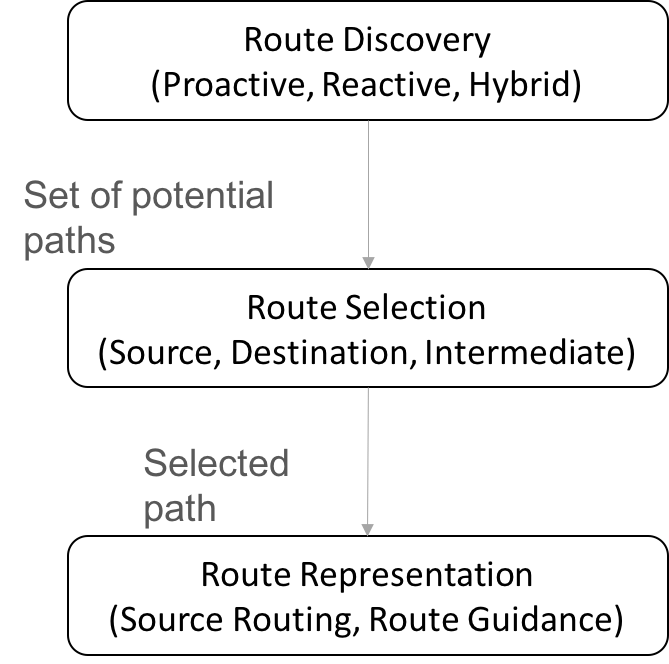
\includegraphics[height =5cm, keepaspectraio]{gfx/RouteFinding.png}
	\caption{Route Finding Phases}
	\label{fig:RouteFinding}
\end{figure}

\begin{enumerate}

    \item \label{enumerate:RouteDiscovery} Route Discovery: Three ways exist to find a route from source to destination:

    \begin{enumerate}
    
    	\item Proactive: Protocols like \ac{DVR} (\cite{RFC1058}) and \ac{OLSR} (\cite{RFC3626}) use pro-active techniques to find a route to the destination. They maintain routing tables to store information about how to reach the destination. Although this technique is quite good for high traffic but it has huge memory requirement to store tables for the entire network.
    	
    	\item Reactive: Protocols in this category, e.g. \ac{AODV} (\cite{RFC3561}) and \ac{DSR} (\cite{RFC4728}), perform on-demand  route discovery by sending a \ac{RREQ}, containing the desired destination address for data sending, to neighbors and receive a \ac{RREP} from the destination. Route discovery can be done in two pays: Firstly, doing it on fly. Under this technique route is searched whenever required. Secondly, it can be done hop-by-hop. In this technique each \ac{SN} decides the next suitable neighbor to forward the packet. \acp{SN} accomplish this task by exchanging periodic routing updates through beacons containing necessary information for neighborhood discovery.
    		
    	\item Hybrid: Protocols combining feature from both, proactive and reactive protocols.

    \end{enumerate}

    \item \label{enumerate:RouteSelection} Route Selection:
    
    For proactive protocols, route discovery phase is sufficient for route selection. Periodically updated routing tables provide the intended nodes with the information about how to reach destination nodes. However, this is not the case with reactive protocols. The selection phase can be handled by either of the three terminals: source, destination or the intermediate nodes.
    
    \par	
    The decision to make source or destination based route selection can depend on the application requirements. Hop count, end-to-end delay/jitter, interference level, packet loss rate, link residual capacity, load balancing and so on can be among the several possible metrics to select the net hop route. In general, number of hop counts to destination is often the preferred metric as it is easy to compute and also it provides us the shortest path to destination. For intermediate nodes, the route selection is done by every node on way to discover the best next hop. 
    
    \item Route Representation:
    
    Two approaches exist to achieve route representation: Either storing the exact route via routing tables/source routing or provide a route guidance. To implement the source routing approach, we need to include the exact route from the source to destination in the \ac{RREP} packet header. The sender then forwards the packet to the next recipient specified in the packet header. This process continues until the packet reaches the destination. In contrast to source routing, the route guidance method involves intermediate nodes to find the best next hop.
    
    In order to make the routing more efficient and to save energy by avoiding route re-computation to destination every now and then in heterogeneity, we will implement the idea of source routing in data transmission phase. In this mechanism we will let the sender know about the exact route to destination via which the data transmission phase should take place. This is discussed in more detail in chapter \ref{ch:Implementation}.
    
\end{enumerate}

%************************************************
\section{Data Collection}
%************************************************

Data collection is primarily used to collect sensor data captured by different \acp{SN} in a \ac{WSN}. The nodes collect information from their surroundings and forward this information to \ac{BS}. Data collected from deployed sensors can be further evaluated or analysed at the sink node or \ac{BS}. The fundamental idea is: generation of data at multiple nodes and collection at one node (called Root node or \ac{BS}). This pattern of flow of data also appears to be converging at one point. Efficient collection and reliable sending is a major challenge in the converging flow of the data. This requires quick adaptation to changes in the network without frequent beacon exchanges (because these exchanges consume considerable amount of energy). \ac{CTP} authors (\cite{TEP:119}) have claimed to solve the issues like reliability, robustness and high data delivery ratios.

\par
Most trivial way to realise this form of data collection is via tree establishment by following the below mentioned points:

\begin{itemize}
    \item Root nodes advertise themselves with hop count value 0 to the neighbors.
    \item Other \acp{SN} collect information like hop distance, node id and more from their neighborhood.
    \item Each \ac{SN} selects one of its neighbor as parent based on certain metrics (for examples refer to \ref{enum:linkqualitymeasures}).
    \item The parent nodes handle and forward the packets received from their children.
\end{itemize}

However there are following issues which also need to be taken care while establishing a tree.

\begin{itemize}
    \item Uni-directional links: A \ac{SN} determines the closest parent as the one which can only send packets but can not receive them.
    \item If a node accidentally receives one beacon from a far away node
    \item Mobile nodes: Node selected as parent is not in range because of it's mobile nature
\end{itemize}

Therefore, while selecting a parent we also include parameters to estimate link quality. Some of the ways to measure link quality are mentioned below:

\begin{enumerate}\label{enum:linkqualitymeasures}
    \item \ac{PRR}: Send a predefined number of packets and measure what fraction of these are received at regular intervals.
    
    \item \ac{RSSI}: Analyze received packets with regard to their signal strength (serving as an indicator for the node distance).

    
    \item \ac{LQI}: Correlation between bits in the \ac{SFD} to indicate potential channel issues (reflection, scattering, etc).

    \item \ac{ETX}: Estimate how many re-transmissions are needed on average when using a particular link.
\end{enumerate}

	
	%************************************************
	\subsection{Collection Tree Protocol}
	%************************************************
	
	\ac{CTP} is a \ac{DVR} protocol. \ac{DVR} is based on the idea of manipulating the vector distances to other \acp{SN} in the \ac{WSN}. Under this routing methodology, each \ac{SN} maintains a routing table consisting of following two information to reach each of the possible final destination \acp{SN}. 
	
	\begin{enumerate}
	    \item next node: Direction in which packet should be forwarded
	    \item cost: Hop counts from the destination
	\end{enumerate}
	
	Every entry in the next node column of the routing table must be an adjacent \ac{SN}, so that the intended sender can directly forward it's packets to this adjacent member. The table is maintained by periodic exchange of the vector consisting of the adjacent node routing table's cost column. Every \acp{SN} updates it's cost column by keeping the minimum of cost value it knows previously and the recently arrived cost vector. To avoid loops in the routing protocol, \ac{CTP} uses datapath validation technique. This technique gets rid of the routing loops by triggering routing updates when it encounters a data packet to be forwarded has lower \ac{ETX} value than it's current \ac{ETX} value or vice-versa or the \ac{ETX} value of a node drops significantly (in \ac{CTP} this threshold is 1.5). \ac{CTP} also uses adaptive beaconing mechanism to minimise power consumption and update stale information. The periodic timer to update stale information goes on increasing exponentially but the timer is reset as soon as the route update request is received. 
	
	\subsection{Implementation}
	
	In \ac{CTP}, \ac{ETX} metric is used to establish a tree topology for data collection. Every node broadcasts beacons indicating its \ac{ETX} to the sink. Broadcast intervals are exponentially increasing (up to 512 seconds), in static network conditions. Further, nodes select their parent based on the \ac{ETX} metric. Nodes compute their \ac{ETX} using the formula: 

    \[ \ac{ETX}_{ToSink} = \ac{ETX}_{Parent} + \ac{ETX}_{Node-ParentLink} \] 

    In this protocol parent can also be updated during run time when link with better \ac{ETX} becomes available. A \ac{SN} participating in \ac{CTP} collection, sends its data as uni-cast messages with link-layer acknowledgments enabled. TinyOS developers have included \ac{CTP} implementation in their operating system libraries. This can be found at \cite{tinyOS:ctpImplementation}. In the following section we will describe the main role taken by the software components of \ac{CTP} framework as shown in figure \ref{fig:CTPFramework}.
	
	\begin{center}
    \begin{figure}[h]
    	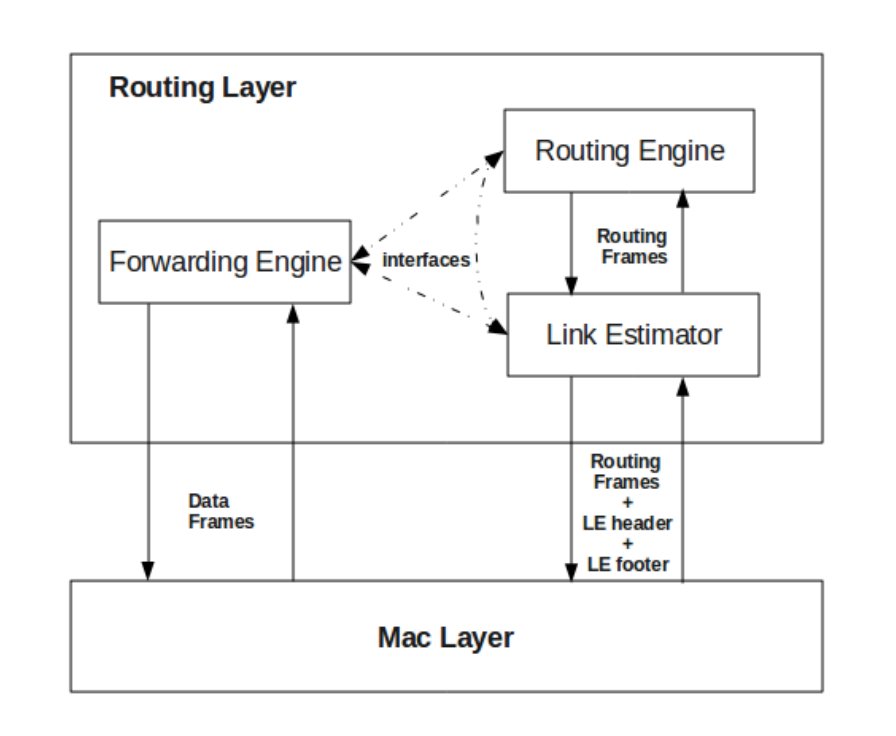
\includegraphics[height=10cm]{gfx/MessageFlowandmodulesInteractions.png}
    	\caption{Message flow and modules interactions, from \cite{colesanti2010performance}}
    	\label{fig:CTPFramework}
    \end{figure}
    \end{center}
	
    \begin{enumerate}
        
        \item Link estimation: This component provides the \ac{ETX} information for one hop communication between two \acp{SN}. This value is updated based on the adaptive beaconing strategy as mentioned in the above section. It also combines information from physical, data link, and network layers to provide accurate link quality estimates. For every 5 transmissions by the \ac{ETX} estimator, it produces an \ac{ETX} value of 6, if the number of successful transmissions is 0. The implementation for this module can be found in \cite{ctp:linkEstimation}.
        
        \item CtpRoutingEngineP: This component provides methods to select the next hop for data transmission based on the \ac{ETX} values obtained from Link Estimator. It also stores the minimum cost route to the root node. A root node advertises it's \ac{ETX} as zero and the \ac{ETX} of a \ac{SN} is calculated by adding the \ac{ETX} of it's parent node plus the \ac{ETX} of the link to it's parent node. 
        
        \ac{CTP} beacons are sent at specific intervals determined by Trickle algorithm. The algorithm allows to gradually reduce the beacon sending rate which further helps in saving energy and bandwidth. However, data path validations can reset this interval to make the \acp{SN} react to topological and environmental changes quickly.
    
        
        \item CtpForwardingEngineP: It is responsible for forwarding the packets received from child nodes as well as the data generated by the \ac{SN} itself. It also attempts retransmissions when necessary (in worst case up to 32 times). It also informs about the routing inconsistencies like routing loops to routing engine. 
        
    \end{enumerate}
    
    
	%************************************************
	\subsection*{CTP for Heterogeneity}
	%************************************************
    
    \par
    We have re-used existing metrics provided by \ac{CTP} for finding solution to best next hop discovery. This can be done by tweaking the routing engine component in \ac{CTP} (which establishes a collection tree to collect data at sink). Moreover, the information provided by \ac{CTP} is a reliable solution to find neighbors and estimate routes because the protocol considers information from link layer and routing layer to estimate the link quality. We will discuss in detail about the modifications and usage of \ac{CTP} in heterogeneity in chapter \ref{ch:Implementation}.

% !TEX root = ../TUCthesis.tex

%************************************************
\chapter{Literature Review}\label{ch:literature}
%************************************************

Several works have been proposed in the direction of extending resource power and achieving higher average energy budget of the sensor nodes across the \ac{SN}. Most of the solutions are scenario specific and do not give good results under altered conditions and assumptions. Pottie and Kaiser \cite{pottie2000wireless} in their paper have stated that transmissions of about 100 metres range is equivalent to 3000 instructions. Therefore, we need protocols for data aggregation or local processing to minimise energy expenses in performing long range transmissions. Local processing of data can be based on two approaches: cluster based mechanism or addition of heterogeneous processing nodes in the network. In this section we will review the existing protocols in these fields and motivate our research work.

%************************************************
\section{Cluster-based}
%************************************************

The concept of clustering to solve the problem of local data processing requires the selected leaders or cluster heads to cater for the communication and processing overhead. Based on the this concept, the paper LEACH \cite{Heinzelman:2000}, was proposed. Though, this algorithm uses randomized cluster head rotation to address the problem of evenly distributing energy load among sensor nodes, yet there are problems in cluster election and cluster formation phase. Also, there is a elevated energy consumption between cluster heads and \acp{BS} as the cluster heads are required to communicate directly with \ac{BS}. In order to directly communicate with the \ac{BS}, the cluster heads will have to send many packets using their high transmission power. Therefore amount of energy dissipated in performing high power transmission will still be a major concern even if we address the problem of fairly assigning slots to the available senders. Improvements to the cluster based algorithms were proposed. LEACH-C \cite{Heinzelman:2002}, which is one of the proposed improvements to LEACH, improves the cluster formation by using a centralized scheme to distribute cluster heads through out the network. More advanced version of LEACH-C was proposed by Zhao in paper \cite{zhao2004energy}. Their algorithm does not require centralised allocation of cluster heads by \ac{BS} and distributes cluster heads more uniformly across the network. 

\par
Projects on hybrid algorithms for clustering like in a paper by Jung \cite{Jung:2009} takes into account several factors like residual energy and distance for adaptive static and dynamic clustering formation for high and low data traffic rates respectively. Many authors like Ye, in the paper EECS \cite{Ye:2005} argue distributed interaction, load-balanced clustering and low-control overhead for data collection. In this mechanism, the larger the distance between cluster head and base station, the smaller member size the cluster head should accommodate to compensate for the penalty of long range transmission. Chain based algorithms like PEGASIS \cite{Lindsey:2002} and CHIRON \cite{Chen:2009} improve the energy efficiency of the network by allowing each node to play the role of head node in turn but still transmission to distant nodes in long chain remains a problem. Since there can be only one node and multiple transmissions are not possible, latency remains an issue for chain-based algorithms. Therefore, it can be concluded that clustering and chaining algorithms can not be used to address the problem significantly.

%************************************************
\section{Heterogeneity}
%************************************************

Adapting heterogeneity to a routing protocol is another way to approach the problem of local data processing with minimal energy consumption. In the paper authored by Sharma and Mazumdar \cite{Sharma:2005}, the focus is on establishing heterogeneity by using wired connections between certain nodes to reduce the overall energy consumption. However, this idea limits the usability of a network for long-term scenarios. in an another work using the Mica2 motes and stargate devices, Hu et al. \cite{hu2009design} have built a hybrid network for detecting cane toads in northern Australia. They have proposed to build a \ac{WSN} with low-power motes with higher processing capabilities. This again puts a limitation to the idea as this would lead to faster draining up of energy because resources consume energy, even if they are not being used. Therefore, they can not be used for autonomous deployments.

Use of mobile agents to carry the code and state information from one device to another has also been studied to address heterogeneity issue. In a paper titled AFME  \cite{muldoon2008agent} and in a similar paper titled: MAPS \cite{Aiello:2011}, authors have explored in the direction of using mobile agents. However, the object-oriented designs of mobile agents are quite slow and extremely difficult to implement.

To increase the network lifetime, Rhee and et. al. \cite{Rhee:2004}, have proposed the use of functional device heterogeneity. The paper is based on the idea of Endpoints, nodes which can not relay data on behalf of others and rather act only as destination for the communication, and routers, nodes that operate with higher duty cycles as they can relay data on behalf of others. In the paper by Yu \cite{Yu:2007}, researchers have supported the idea of optimizing the number and location of processing nodes, which lies more in the domain of a Mathematical Optimization.

\par
From the theoretical energy analysis, Reinhardt and et. al. in their paper \cite{reinhardt2013exploiting}, have concluded that heterogeneous \acp{SN} are beneficial to deploy in a network with three major application scenarios: cryptography, compression and high-data rate processing within the \ac{WSN}. From the evaluation, they have come to a conclusion that: "Energy savings can be achieved by deploying processor nodes, as their greater energy consumption is counterbalanced by reduced execution times and less traffic in the network." 

In a similar work by Reinhardt and et. al. \cite{reinhardt2008designing}, they have argued that platform heterogeneity with task migration concept can save the overall energy budget of a \ac{WSN}. They have reasoned this with task migration concept which can play a part in the \ac{WSN} when the energy demand for transmission of data plus remote processing is less than local processing of data plus estimated energy demand of processing and reception of data. 

Our paper focuses on abridging the research gap on simplified deployment of heterogeneity in a \ac{WSN} which is based on the idea of energy savings as proposed in paper \cite{reinhardt2013exploiting} by minimising the number of transmissions required to deliver the data to the \ac{BS}. Our aim is to address the drawbacks and limitations of heterogeneity concept and further propose a simplified mechanism to provide the heterogeneity layer as an additional plug in on top of the selected routing protocol. Since heterogeneity layer has to depend on other routing algorithms to get the data delivered to \ac{BS}, we simulate heterogeneity on top of \ac{CTP} algorithm, which is considered robust, reliable and efficient for diverse number of platforms. In the paper \cite{pecho2010simulation}, the authors have concluded that \ac{CTP} is designed for low data rates. Our work on heterogeneity also aims to extend \ac{CTP} for high data transfer rates. therefore, the heterogeneity layer should also be seen as an extension to increase the overall flow of wireless data traffic at minimal energy expenditure. 



% !TEX root = ../TUCthesis.tex

%************************************************
\chapter{Implementation of Heterogeneous WSN}\label{ch:Implementation}
%************************************************

The \acp{SN} in the heterogeneity network model are not centrally operated to avoid single point of failure. Therefore they act independently to co-ordinate and communicate with their neighbors to resolve contentions among the \acp{SN} for heterogeneity layer access. This approach requires frequent message exchanges among the nodes. Therefore, we need an efficient routing methodology to minimise the beacon exchange count and further initiate the data transfer via heterogeneity in a contention free slot. 

In order to realise the benefits of deploying heterogeneity in a network, we simulate heterogeneity along with \ac{CTP} algorithm. This chapter describes the simulation methodology and programming structure of heterogeneity concept. In the first section, Platforms used \ref{sec:PlatformsUsed}, we describe the hardware and software components used for simulating the network model. In the second section, Design Components \ref{sec:DesignComponents}, we provide an overall picture of heterogeneity model and further describe the TinyOS components and interfaces involved in the design phase. This also explains the importance of \acp{CTP} module for our routing model. In the third section, Control Plane Design \ref{sec:ControlPlaneDesign}, a detailed analysis of the routing mechanism in heterogeneity is provided. It describes three aspects of heterogeneity: 1. how the protocol finds the route to destination heterogeneous node 2. the criterion to decide one of the possible routes found by route discovery phase 3. how the final selected route is represented in the heterogeneity model. As a follow up to the routing model, the subsection, Routing Implementation, conforms the routing model requirements with heterogeneity model. This subsection also contains the packet contents of message exchanges in heterogeneity. The packets in our network model serve as an important aspect to realise information exchange among \acp{SN}. In the fourth section, Heterogeneity Specific Implementations \ref{sec:heterogeneitySpecificImplementations}, we provide a detailed explanation of data structures involved in running the heterogeneity model. The explanation focuses on two major aspects: 1. how these data structures are linked to each other and 2. how their interdependency act as an important tool to regulate state change in heterogeneity. In the fifth section, Data Plane Design \ref{sec:DataPlaneDesign}, data transmission in one hop and two hop neighborhood through heterogeneity is explained. In the final section \ref{sec:processModel}, we present the flow diagrams to sketch the life cycle of heterogeneity model. 

%************************************************
\section{Platforms Used} \label{sec:PlatformsUsed}
%************************************************

This section is divided in two parts: hardware components and software components.

    %************************************************
    \subsection{Hardware Components}
    %************************************************
    
    The hardware used for implementation are Telosb motes \cite{datasheet:Telosb}. This sensor platform was originally developed by the University of California, Berkeley by TinyOS developers. It features the 8MHz Texas Instrument MSP430 (the MSP430F1611) microcontroller with a 10 kBytes internal RAM and a 48 kBytes program Flash memory, IEEE 802.15.4 CC2420 radio chip, data transfer rate up to 250kbps, integrated onboard antenna, 1MB external flash for data logging, programming and data collection via USB, sensor suite including integrated light,  temperature and humidity sensor and runs on TinyOS 1.1.10 or higher.
    
    %************************************************
    \subsection*{MSP430 Microcontroller}
    %************************************************
    
    The MSP430 \cite{website-MSP430} is a low-cost microcontroller generally used for low powered embedded devices. It has a 16-bit \ac{RISC} CPU with an instruction cycle time of 125$nS$. The device is highly optimised for low energy consumption and high code efficiency. It supports six different low-power modes to disable unnecessary running of clocks and CPU. It is capable of wake-up times below 1$\\muS$, which allows the microcontroller to stay in low power mode for longer period of time and thus maximising the available energy budget. The power consumption in active mode is about 330$\mu A$ at 1MHz with 2.2V. In idle mode the microcontroller needs less than 1$\mu A$. The supply voltage should be in the range of 1.8V to 3.6V.
    
    %************************************************
    \subsection*{CC2420 Radio}
    %************************************************
    
    It is a 2.4GHz IEEE 802.15.4 complaint RF transceiver  \cite{TI:cc2420}. It is specially designed for low power embedded devices. Some of the important features include: extensive hardware support for packet handling, data buffering, burst transmissions, data encryption, data authentication, clear channel assessment, link quality indication and packet timing information.
    
    %************************************************
    \subsection{Software Components}
    %************************************************
    
    We have compiled our heterogeneity code in TinyOS which uses nesC programming language. In addition to this, we have also used COOJA simulator \cite{cooja:Contiki} to simulate the compiled code in a virtual \ac{WSN} environment. Cooja is a java based simulator for emulating \acp{SN} of certain platforms at hardware level. This allows faster and precise inspection of the model behaviour for the compiled TinyOS code.

%**********************************************************
\section{Design Components} \label{sec:DesignComponents}
%**********************************************************
In the first subsection, we will discuss heterogeneity implementation possibilities with a focus on energy and computational power. In the second part, we will briefly explain about the working of heterogeneity layer and in the final subsection, we will talk about the general TinyOS components required for implementing heterogeneity.

    %************************************************
    \subsection{Heterogeneity Possibilities}
    %************************************************
    
    From the literature survey in chapter \ref{ch:literature}, we have explored several possible dimensions of  heterogeneity implementation including increased energy, computational power, memory, wireless range, etc. for a particular group of \acp{SN}. With \acp{CTP} being the most widely used protocol, we implement it as the baseline for collecting data generated at a \acp{SN} and for the sake of simplicity, we rely on the parameters energy and computational complexity throughout the remainder of the report. Also, we depend on these parameters to perform a comparative analysis of heterogeneity with \acp{CTP}.
    
    %************************************************
    \subsection{Outline}
    %************************************************
    
    The heterogeneity set up requires \ac{CTP} implementation (provided in \cite{tinyOS:ctpImplementation}) at back end. \ac{CTP} is responsible for building and maintaining minimum cost trees to nodes which advertise themselves as roots based on \ac{ETX} parameter. Messages are sent and received via \ac{CTP} send and receive interfaces. On top of the \ac{CTP} layer, we implement the heterogeneity layer. The tasks performed by this layer are sequential and event-driven. \acp{SN} respond to different events and thus change their states on subsequent events reception or triggering. We will discuss more about states and flow diagrams in section \ref{sec:processModel}. These states are stored as global variables  or well-defined structs in the implementation. In summary, the \acp{WSN} operates in an endless loop in the following order:
    
    \begin{enumerate}
        \item Beacon based \ac{PC} announcement in one and two hop neighborhood: Each \ac{PC} participates in the periodic advertisement of their computational power availability to their one and two hop neighbors.
            
        \item Selective \ac{RTS} response by \ac{SN} to the beacon announcement: The notion of \ac{RTS} concept used in heterogeneity layer is equivalent to sending a request packet to check the \ac{PC} availability before the actual transmission of data. The packet requests a unique time slot for the intended sender and thus resolves the conflict of multiple data senders to one \ac{PC}.
        
        \item \ac{CTS} response by \ac{PC}: Based on the earliest \ac{RTS} request, a \ac{CTS} response is generated by the \ac{PC} for the intended sender. The notion of \ac{CTS} response implies that the \ac{PC} will have to send a clear to send signal before the intended \ac{SN} can initiate the data transmission. Until the intended sender gets a \ac{CTS} response, it participates in \ac{CTP} collection for sending it's data.
        
        \item Data transfer via heterogeneity layer: On reception of \ac{CTS} response by the intended sender, the data transmission phase starts for the time period the intended sender requests. 
        
        \item Data collection via \ac{CTP} from \ac{PC} to \ac{BS}: On completion of data sending by a \ac{SN} to \ac{PC}, the final computed data is added to the data collection queue and thus it reaches the \ac{BS} via \ac{CTP}.
    \end{enumerate}
    
    We will have a closer look at the detailed implementation of the heterogeneity set up in the coming sections and subsections. 
    
    %************************************************
    \subsection{TinyOS Components}{\label{subsec:tinyOSComponents}}
    %************************************************
    
    In this subsection, we will discuss about the interfaces and wiring required for implementing heterogeneity.
    
    \begin{enumerate}
        \item General Interfaces: Following are the commonly used interfaces required for the implementation: 
    
            \begin{itemize}
                \item Boot: It is required to boot a \ac{SN}. the boot interface signals Boot.booted() event on successful booting of the device.
                
                \item SplitControl: It is used to start and stop services of the radio transceiver. It is wired to ActiveMessageC component.
                
                \item StdControl: This interface is provided by Collection protocol. StdControl interface  controls the state of \ac{CTP} routing by setting/resetting the routing state once the routing layer of \ac{CTP} starts or stops respectively.
                
                \item Leds: This is used for controlling the led lights on the Telosb. We use light patterns to indicate transmissions and receptions in our application. The interface is wired to ledsC component and provides methods such as LedsToggle, LedsOn or LedsOff for the leds.
            \end{itemize}
        
        \item CTP-based Interfaces: These interfaces are provided by \ac{CTP} to send and receive messages via the collection tree. 
        
            \begin{itemize}
                \item RootControl: This interface is used to advertise a particular \ac{SN} as a root node of the \ac{CTP} tree.
            
                \item {\label{item:Send}} Send: It is used to send messages via \ac{CTP} protocol through the collection tree. This interface is wired to CollectionSenderC component provided by \ac{CTP}.
                
                \item Receive: It is used to receive messages sent via Send interface in \ref{item:Send}. The messages received via this interface are exclusively sent via \ac{CTP} protocol. Messages sent via other sending interfaces, which are not wired to CollectionSenderC, do not get routed via \ac{CTP}. This distinction helps in implementing an abstraction layer over \ac{CTP} on which we will build our heterogeneity model and thus keep our data exchange model separate from \ac{CTP} communications.
                
                \item CtpInfo: This interface provides methods to obtain \ac{ETX} information about the current \ac{SN}. It is also wired to CollectionC component of \ac{CTP} so that we could obtain the \ac{ETX} metric used in setting up the collection tree. This metric is also updated periodically by \ac{CTP} and therefore keeps the heterogeneity model remians up to date with changes in \ac{ETX} metric.
                
                \item Timer: This timer is fired to perform routing via \ac{CTP}. Only when this timer is fired, the \ac{SN} announces itself as a part of \ac{CTP} and further acknowledges itself as a member of \ac{CTP} tree. 
            \end{itemize}
    \end{enumerate}
        
%************************************************
\section{Control Plane Design } \label{sec:ControlPlaneDesign}
%************************************************
    
This section describes the advertisement phase of a \ac{PC} and \ac{PC} selection phase of an intended sender. We will first describe the routing model and then explain the routing implementation phase of our design.

    %************************************************
    \subsection{Routing Model}
    %************************************************
    
    In this subsection, we will look at the route discovery, route selection, route representation and data forwarding phases of heterogeneity.
    
    \begin{enumerate}
        \item Route Discovery: To derive the route discovery mechanism implemented in our design, we will continue from the previous description on route discovery in section \ref{enumerate:RouteDiscovery} (in chapter \ref{ch:Background}). 
        
        \par
        In our heterogeneity model, we perform the route discovery phase by maintaining an array of known \acp{PC} in at most two hop neighborhood. Therefore, We can say that the route discovery is done proactively because we know exact route from sender to \ac{PC} in advance. A sorting algorithm periodically sorts this array for the optimal selection of \ac{PC} at constant run time ($O(1)$) (explained in detail in sections  \ref{item:routeSelection} and \ref{sec:heterogeneitySpecificImplementations}). Further, to ensure collision free data transmission, a \ac{RTS} packet is sent to the first member of the \ac{PC} array to verify if the recipient is free. 
        
        \par
        The \ac{PC} reply packet carries routing information to stimulate data transmission by sender. We can utilize the concept of message pools to avoid the \ac{PC} route reply packet transmission. The concept of message pool can be exploited in two ways: either we maintain separate queue for each of the possible senders or accept data from all possible senders in one queue at any point of time. Although these methods solve the problem of sender fairness, yet these pools can be memory intensive in high traffic scenario. Also, to implement the latter scenario, we will first have to sort similar data in the message pool and then process them in ordered way. One more drawback of pooling approach is frequent back-offs while sending stream of data because multiple nodes will try to to get channel access while sending to one \ac{PC} and hence would not get clear channel assessment very often. This can finally lead to low data delivery ratio. Therefore, instead of this pooling approach, we have chosen to reserve the processing center for a particular \ac{SN} and only after the reservation confirmation, the intended sender can send their data for processing. We also assume here that each of the \ac{SN} can send only one type of data for the allotted reservation period. A \ac{PC} confirms its own reservation via \ac{RREP} packet to the sender on first come first serve basis. It waits for a certain amount of time to receive data. In case of no reception after passage of allotted time period, it again starts flagging itself as an available \ac{PC} to the \acp{SN} in one or two hop neighborhood. 

        \item \label{item:routeSelection} Route Selection: In the previous discussion on route selection in \ref{enumerate:RouteSelection} (in chapter \ref{ch:Background}), we have explained the possible ways of route selection. Now, we will discuss how we achieve this in our heterogeneity design.
        
        \par
        We use \ac{CTP} to get \ac{ETX} information of the \ac{SN} in order to select the best \ac{PC} for data transmission. As claimed by the authors, \ac{CTP} maintains an updated \ac{ETX} estimate of \acp{SN} on periodic basis. We use these updated \ac{ETX} values for \ac{PC} selection. To extract the \ac{ETX} values, the interface 'CtpInfo.nc' is wired to CTPRoutingEngineP component, which is also provided in the TinyOS \ac{CTP} implementation. This interface provides following useful methods for neighborhood discovery and route selection:
        
        \begin{enumerate}
        	\item getParent() -> Gets the parent of the node in the tree.
        	
        	\item getEtx() -> Gets the \ac{ETX} for the current path to the root through the current parent.
        	
        	\item triggerRouteUpdate() -> Informs the routing engine that sending a beacon soon is advisable.
        	
        	\item numNeighbors() -> Gets number of neighbours.
        	
        	\item getNeighborLinkQuality() - Gets the Link Quality of a neighbor. 
        	
        	\item getNeighborAddr() -> Gets the address of the neighbor.
        \end{enumerate}
        
        \par
         For the route selection process, we propagate the \ac{ETX} information, obtained by  \textbf{getEtx} method, during the beacon broadcasting phase. This value is then used through out in our design and is the building block of optimal \ac{PC} selection. We therefore believe that re-using and keeping an updated copy of this information in the network enhances the network reliability.
        
        \par    
        We have also added an extra method in CTPInfo interface to acquire addresses of all the \acp{SN} in one hop neighborhood. This was done with the help of \textbf{getNeighborAddr} method. This method returns the address of all the \acp{SN} from it's routing table. As mentioned in previous section on route discovery, each \ac{SN} in \ac{CTP} maintains a routing table of size number of neighbors containing neighbor address and other relevant fields. We therefore exploit this routing table information by iterating through all the routing tables for the number of neighbors in one hop neighborhood (provided by CtpInfo numNeighbors method). Further, we store all the neighbor addresses in an array and return it. Although this method is currently not used in the model, but it can be quite useful in improving the network reliability and efficiency by precisely determining the \ac{SN} density around each of the \acp{SN} and further placing a \ac{PC} around it.   
        
        \item Route Representation: We have implemented the idea of route guidance in search phase. However, to make it more efficient, we have blended in the idea of source routing in data transmission phase. This approach will inform the sender about the exact route to destination through which the data transmission phase should take place. In this way we will not waste energy in re-computing the route to destination every now and then. There is also an added benefit to this approach: we do not need to maintain long routing tables as we need only the routing information from the \ac{SN} to the \ac{PC} in one or two hop neighborhood. We therefore do not add routing information for \acp{PC} located at a distance more than two hop and hence avoid maintaining long routing tables and thus leave off the distant \acp{PC}.
        
        \item Auxiliary Components: Apart from the above three routing components, we have also looked into the following aspects: 
    
        \begin{enumerate}
        	\item Route Maintenance
        	\item Route Refreshing
        	\item Route Failure Handling
        	\item Route Invalidation
        	\item Restricted Flooding
        	\item Data Aggregation
        \end{enumerate}
        
        The first four auxiliary components have already been taken care of by re-using the information from \ac{CTP} protocol because the protocol sends beacons every 5ms to update stale route information, if any, in the \ac{WSN}. Also, we have restricted flooding to two hop neighborhood in the route discovery phase. In other phases, we perform unicast transmissions. Moreover, the concept of heterogeneity relies on the notion of data aggregation technique as we send only same type of data to the processing center. This reduces the number of packets flowing through the network which in turn would reduce the overall energy budget of the \acp{SN}.
    
        
    \end{enumerate}
    
    
    %************************************************
    \subsection{Routing Implementation}
    %************************************************
    
    The routing implementation is summarised in following points: 
    
    \begin{enumerate}
        \item As discussed before, route discovery phase begins with beacon advertisement of \acp{PC}. Each node maintains a local copy of the advertising \acp{PC} and use it for route computation phase. Table \ref{tab:Beacon_advertisement} shows the packet contents of beacon advertisement message. 
        
        \begin{table}[h]
    	\caption{Beacon Advertisement} % title name of the table
    	\centering
    	\begin{adjustbox}{max width=\textwidth}
    	
        	\begin{tabular}{|c|c|c|c|} 
        		\midrule
        		Field names: & \ac{PC} ID & \ac{PC} \ac{ETX} &Relayer \ac{ETX} \\
        	    
        	    TinyOS Data Type: & nx\_uint8\_t & nx\_uint16\_t & nx\_uint16\_t \\
        	    
        	    Size(In bytes): & 8 & 16 & 16 \\
        			
        		\hline
        		\end{tabular}
    	\end{adjustbox} 	
    	\label{tab:Beacon_advertisement}
        \end{table}
    
        \item In the next step, a route is selected based on \ac{ETX} values propagated during beacon advertisement.
        
        \item Based on \ac{PC} availability at different moments, we can expect \ac{PC} availability issues. Therefore, we can not rely on static routing table and rather need to determine if the processing centre is available before data transmission. If no \ac{PC} is found free, the data transmission takes place via \ac{CTP}. For determining the availability, the sender sends a \ac{RREQ} to \ac{PC} and in response the \ac{PC} makes a \ac{RREP} to the sender if it finds itself free. Table \ref{tab:CTS_Packet} and shows the contents of \ac{RTS} and \ac{CTS} packets respectively.
        
        \begin{table}[h]
    	\caption{RTS Request Packet} % title name of the table
    	\centering
    	
    	\begin{adjustbox}{max width=\textwidth}
    	\begin{tabular}{|c c c c c|} 
    	
    		\midrule
    		Field names: & Duration & Sender Address & Relayer Address & \ac{PC} Address \\
    		
    	    TinyOS Data Type: & nx\_uint8\_t & nx\_uint8\_t & nx\_uint8\_t & nx\_uint8\_t \\
    		    
    	    Size(In bytes): & 8 & 8 & 8 & 8\\
    			
		\hline
		\end{tabular}
    	\end{adjustbox}
    	\label{tab:RTS_Request_Packet}
        \end{table}
        
        \begin{table}[h]
    	\caption{CTS Response Packet} % title name of the table
    	\centering
    	
    	\begin{adjustbox}{max width=\textwidth}
    	\begin{tabular}{|c c c c c|} 
    	
    		\midrule
    		Field names: & Duration & Sender Address & Relayer Address & \ac{PC} Address \\
    		
    	    TinyOS Data Type: & nx\_uint8\_t & nx\_uint8\_t & nx\_uint8\_t & nx\_uint8\_t \\
    		    
    	    Size(In bytes): & 8 & 8 & 8 & 8\\
    			
    			\hline
    		\end{tabular}
    	\end{adjustbox}
    	\label{tab:CTS_Packet}
        \end{table}
        
    \end{enumerate}

    \par 
    

% heterogeneity layer discovers routes, selects that  

% receive event is rather different than most events: it has a message t* as both a parameter and a
% return value. When the communication layer receives a packet, it passes that packet to the higher layer
% as a parameter. However, it also expects the higher layer to return it a message t* back. The basic idea
% behind this is simple: if the communication layer doesn’t have a message t*, it can’t receive packets, as it
% has nowhere to put them. Therefore, the higher layer always has to return a message t*, which is the next
% buffer the radio stack will use to receive into. This return value can be the same as the parameter, but it does
% not have to be. A receive handler can always copy needed data out of the packet and just returned the passed buffer.

% How tinyos operates in general:

% An event driven operating system with blocking mode?

% How does it interface with multiple devices and support them?

% What generalisation it offers to multiple platforms?

% Design patterns with TinyOS?
    
%     Available Data structures
    
%     Limitations in Data structure which makes coding efficiency a problem 


%************************************************
\section{Heterogeneity Specific Implementations}\label{sec:heterogeneitySpecificImplementations}
%************************************************
 In the following subsections, we will describe heterogeneity specific design data structure and further point out two important elements of this design: Periodic Member Updating and Periodic Sorting.
    %************************************************
    \subsection{Data Structures}
    %************************************************
        \begin{enumerate}
            \item Enums: They are used as constants for defining timer intervals, debug parameters, ids of the \acp{PC} and \ac{BS}, random data transfer duration selection for each \ac{SN} and many other parameters used in the simulation.
            
            \item Queues: TinyOS Queue interface is equivalent to a Queue data structure. Important commands in this structure include commands to en-queue an element, de-queue an element and retrieve queue size. In heterogeneity, we have implemented following four queues:
            
                \begin{enumerate}
                    \item CTSQueue: This queue stores \ac{RTS} requests from the intended data senders to the \ac{PC}. This has been defined as a queue to store multiple \ac{RTS} requests to the \ac{PC} and further send out the \ac{CTS} response to one of them based on a specific criterion. Although in the current implementation we have sent out the \ac{CTS} response on first come first serve basis, and thus the idea to store multiple \ac{RTS} requests may not seem much useful but for future testing and comparative studies, we can choose an optimisation algorithm to send out the \ac{CTS} response based on parameters like: fairness, \ac{ETX} or other \ac{LQI}. This has been done to make the heterogeneity layer extensible to other \ac{WSN} application domains. 
                    
                    \item DataStoreQueue: This queue holds the data transfer information of the \acp{SN} which are participating in data transfer phase of heterogeneity. Every member of this Queue is a struct of \ac{PC} id, Relayer id, Sender id, and the data transfer duration approved by \ac{PC}. As soon as the recipient confirms its id with the \ac{CTS} response, it en-queues itself in the queue and calls data transmission phase to initiate the data sending operation.
                    
                    \item DataGenerationQueue: This queue stores data for transmitting it through collection tree formed via \ac{CTP}. Principally, each \ac{SN} generates data on a periodic basis, which has to be de-queued and further sent out via \ac{CTP}. However, if a \ac{SN} is granted \ac{CTS} permission to send data to the \ac{PC}, the node stops sending it's data via \ac{CTP} and instead de-queues data from the DataGenerationQueue and forwards them to the \ac{PC} via heterogeneity layer.
                    
                    \item CTPCollectionDataQueue: This queue holds the processed data collected from the heterogeneity layer. On receiving the data termination beacon from the sender node, the \ac{PC} processes the incoming data and enqueues it in this queue. Further it gets collected via \ac{CTP}.
                    
                \end{enumerate}
            
            \item Structures: Following structures are used in the application:
            
                \begin{enumerate}
                    \item beaconBroadcastMsg: \acp{PC} broadcast out their availability to at most 2hop neighbors. This message is forwarded as a network packet containing \ac{ETX} and id of \ac{PC}. Later the relayer adds its own \ac{ETX} to the packet, when the message is finally forwarded out to two hop neighbors of \ac{PC}.
                    
                    \item{\label{item:processingCentreStruct}} processingCentre: This array of structure holds the information of the processing centers in it's 1hop or 2hop neighborhood as an individual member. The information includes ids and \ac{ETX} of \ac{PC} and relayer. This information is updated after a \ac{SN} receives broadcasting beacons from the \ac{PC} in one or two hop neighborhood. If the Process centre is in the immediate one hop then the relayer is by default set as 0. \acp{SN} scan this array to find out the most suitable processing centre in it's neighborhood for sending \ac{RTS} request. This scanning also filters out the nodes indicated as busy in busySensorNode array (\ref{item:busyNode}).
                    
                    \item PreambleMsg: This is sent out as a network packet as \ac{RTS} in response to \ac{PC} availability indicated by beaconBroadcastMsg broadcasted by \ac{PC}. 
                    
                    \item{\label{item:busyNode}} busySensorNode: Every node maintains a copy of busy \acp{SN} in it's neighborhood. This array of struct holds, ids of busy \acp{PC}, relayers, senders and time period allotted for the intended sender to transfer data, as an individual member of the struct array. This information is kept up-to date via a periodic timer which keeps on decrementing the time period allotted at every firing interval. After the allotted time period reduces to zero, the structure member is remove from the array of structs.
                    
                    \item dataSendStruct: In the data transmission phase, the sender sends out the data and packet counter (for debugging purposes) to the \ac{PC} which has sent the sent a \ac{CTS} response.
                    
                \end{enumerate}
                
        \end{enumerate}
    
    %************************************************
    \subsection{Periodic Member Updating}
    %************************************************
    
    We rely on periodic \ac{CTP} control beacons to update the stale ETX information for each of the member node. At heterogeneity layer, we update \ref{item:processingCentreStruct} on periodical beacon announcements by \acp{PC}. These beacons indicate the availability of \ac{PC} in at most 2hop neighborhood. We also understand that this periodic update is not necessary so often if the \ac{PC} is already included in the array. Therefore we also put a minimum number of beacons received on updating a stale member of the struct. This approach resolves the trade-off between accurate data availability and low cost. The heterogeneity layer updates the \ref{item:processingCentreStruct} on two occasions:
    
    \begin{enumerate}
        \item It receives a beacon from an unknown \ac{PC}. As a result of the reception, the new member is appended in the array.
        
        \item It receives a beacon from a known \ac{PC}. In this case, the member is only updated after the enumerate E\_MEMBER\_UPDATE\_PERIOD reaches it's maximum count.
    \end{enumerate}
    
    %************************************************
    \subsection{Periodic Sorting}
    %************************************************
    
    Periodically, the members in \ref{item:processingCentreStruct} are sorted in the descending order of priority. The sorting depends on the following parameters:
    
    \begin{enumerate}
        \item Lowest \ac{ETX} value within 1hop neighborhood (the relayer value is zero)
        \item Lowest \ac{ETX} value within 2hop neighborhood (the relayer value is non-zero)
    \end{enumerate}
    
    \par
    This sorting helps in selecting the best \ac{PC} in $O(1)$ run time. This sorting is useful in situations where there are short data transfer slots and frequent re-assignments of \acp{PC} to the \acp{SN}. However, in situations where we have longer data transfer durations implying sporadic re-assignments of \acp{PC}, it is worth removing the timer and instead calling this sorting method on-demand (when \ac{RTS} has to be sent to \ac{PC}).   

%************************************************
\section{Data Plane Design}\label{sec:DataPlaneDesign}
%************************************************

On reception of \ac{CTS} packets from the \ac{PC}, DataSendingTimer is fired to trigger the data sending phase for intended sender. During this period, the \ac{PC} marks itself as busy, stops advertising itself as \ac{PC} in two hop neighborhood and does not further respond to any \ac{RTS} requests. DataSendingtTimer sends out three beacons preceding the actual data transmission to indicate the beginning of data transmission phase and at the end of data transmission phase it again sends out three beacons to indicate the termination of data transmission phase. This process is necessary in the data transmission implementation to precisely determine the actual start and end time of data transmission phase. On successful reception of at least one of the termination beacons, other received termination beacons are simply ignored. We also need to send out more than one beacon to let the \ac{PC} know that data sending has been terminated because the \ac{PC} has to precisely know when it has to en-queue the computed data in I\_CTPCollectionDataQueue. Also sending out only one beacon has more sending or receiving failure probability due to multiple channel back-offs or receiving event errors at \ac{PC}. Therefore, this failure can discard the entire data which was received but not processed and hence not en-queued for collection via \ac{CTP} after the data transmission had completed. 

\par
This will be discussed in more detail in following two subsections. The first part covers the case for data sending in one hop neighborhood and the second part covers the data sending operation via a relayer to a two hop \ac{PC}.

	%************************************************
	\subsection{One-hop Data Transmission}
	%************************************************
	
    Data sending in one hop is straight-forward. We use AMSend interface to send data to the \ac{PC}. In this case the \ac{PC} is set as the destination address in the \textit{AMSend.send} method. The relayer address is set to zero because we do not need a relaying point to forward our data. The sender sends data via a specific instance of AMSend interface (instantiated via an integer am\_id\_t) and the \ac{PC} receives them via AMReceieve event parametrised to same am\_id\_t as that of sender. This transfer takes place for the duration of transfer requested by intended sender minus a small safe margin value to compensate \ac{RTS} and \ac{CTS} beacon exchange period. Finally, on reception of termination beacons, the \ac{PC} does some complex computation on the received data and en-queues it in I\_CTPCollectionDataQueue for data collection via \ac{CTP}.
	
	%************************************************
	\subsection{Two-hop Data Transmission}
	%************************************************
    
    Data sending in two hop is more complicated than one-hop transfer. On reception of \ac{CTS} response, both the sender and relayer mark themselves as busy. The relayer on reception of data always checks who the data is intended to from the packet contents. It extracts the \ac{PC} address from the packet contents and forwards the data to the extracted \ac{PC} address. Now, for the \ac{PC}, which is also the two hop recipient, the data appears to be forwarded as one hop traffic from relayer. The \ac{PC} further en-queues the collected data in I\_CTPCollectionDataQueue on reception of termination beacons.
                
	%************************************************
	\subsection{Data Processing Phase}
	%************************************************
	
    The incoming data from sender is processed on each packet reception. On reception of data from the intended sender, the \ac{PC} serially forwards it to a heterogeneous device (such as Raspberry Pi or a computer) over usb connection. We had motivated the need of heterogeneity (in chapter \ref{ch:introduction}) for running memory intensive and/or computation intensive algorithms like data compression, Fourier transform, data analysis on the \ac{PC}. We can implement these algorithms on the attached peripheral and forward the incoming data serially to the heterogeneous device. We would like to mention here that data processing power of a \ac{PC} entirely depends upon the computational capabilities of the peripheral component.

%************************************************
\section{Process Model}\label{sec:processModel}
%************************************************

Our model works on the systematic calling of timers when required. Some of these timers follow periodic patterns while others are called when certain conditional elements are encountered. For the conditional timers, the timer is called once by \textit{Timer.StartOneShot} method and this calling repeats in a loop until the condition to execute the loop holds. In the following subsections we will describe these timers and conditional elements to keep these timers running.

	%************************************************
	\subsection{System Overview}
	%************************************************
	
	The work flow of heterogeneity model is illustrated using the figure \ref{fig:TimerWorkflowSummarised}. This work flow is further briefly discussed in following points:
	
	\begin{enumerate}
	    \item BeaconTimer: This is a periodic timer fired by \acp{PC}. On firing of the timer, a \ac{PC} advertises itself as the available processing device centre in two hop neighborhood.
	    
	    \item This advertisement is updated and sorted locally by each \ac{SN} periodically by SortProcessingCentreBasedOnETX timer.
	    
	    \item Intended sender nodes use the best available \ac{PC} and sends \ac{RTS} request using PreambleSendingTimer.
	    
	    \item The \ac{PC} replies to the \ac{RTS} via \ac{CTS} messages.
	    
	    \item \acp{SN} snoop the \ac{CTS} response and update their Busy \acp{PC} and relayers struct array.
	    
	    \item On receiving \ac{CTS} response by the intended sender, DataSendingTimer is fired and data transmission phase starts.
	    
	    \item On completion of data transmission, CTPCollectionTimer collects this data and sends its via \ac{CTP} to \ac{BS}.
	    
	    \item In case of no \ac{PC} availablity in one or two hop neighborhood, the \ac{SN} participates in the \ac{CTP} forwarding of data via CTPCollectionTimer.
	\end{enumerate}
	
	\begin{figure}
    \centering
    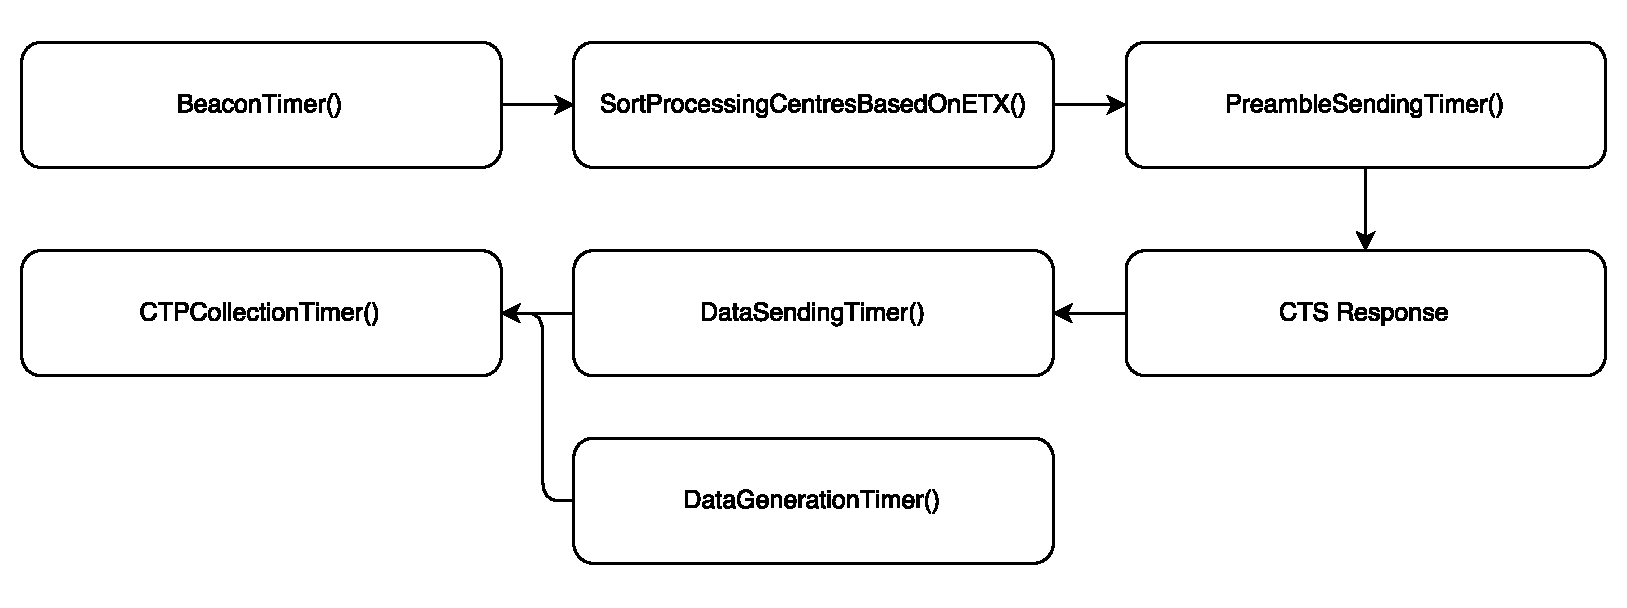
\includegraphics[width=1.0\textwidth]{gfx/TimerWorkflowSummarised.pdf}
    \caption{Timer Work Flow Summarised}
    \label{fig:TimerWorkflowSummarised}
    \end{figure}
	
	In subsection \ref{subsec:TimersFlowchartDiagrams}, we will differentiate the timers for different types of \acp{SN}. And in the further subsections we will discuss these timer

	%************************************************
	\subsection{Timers Flowchart Diagrams}\label{subsec:TimersFlowchartDiagrams}
	%************************************************
	
	\begin{figure}
    \centering
    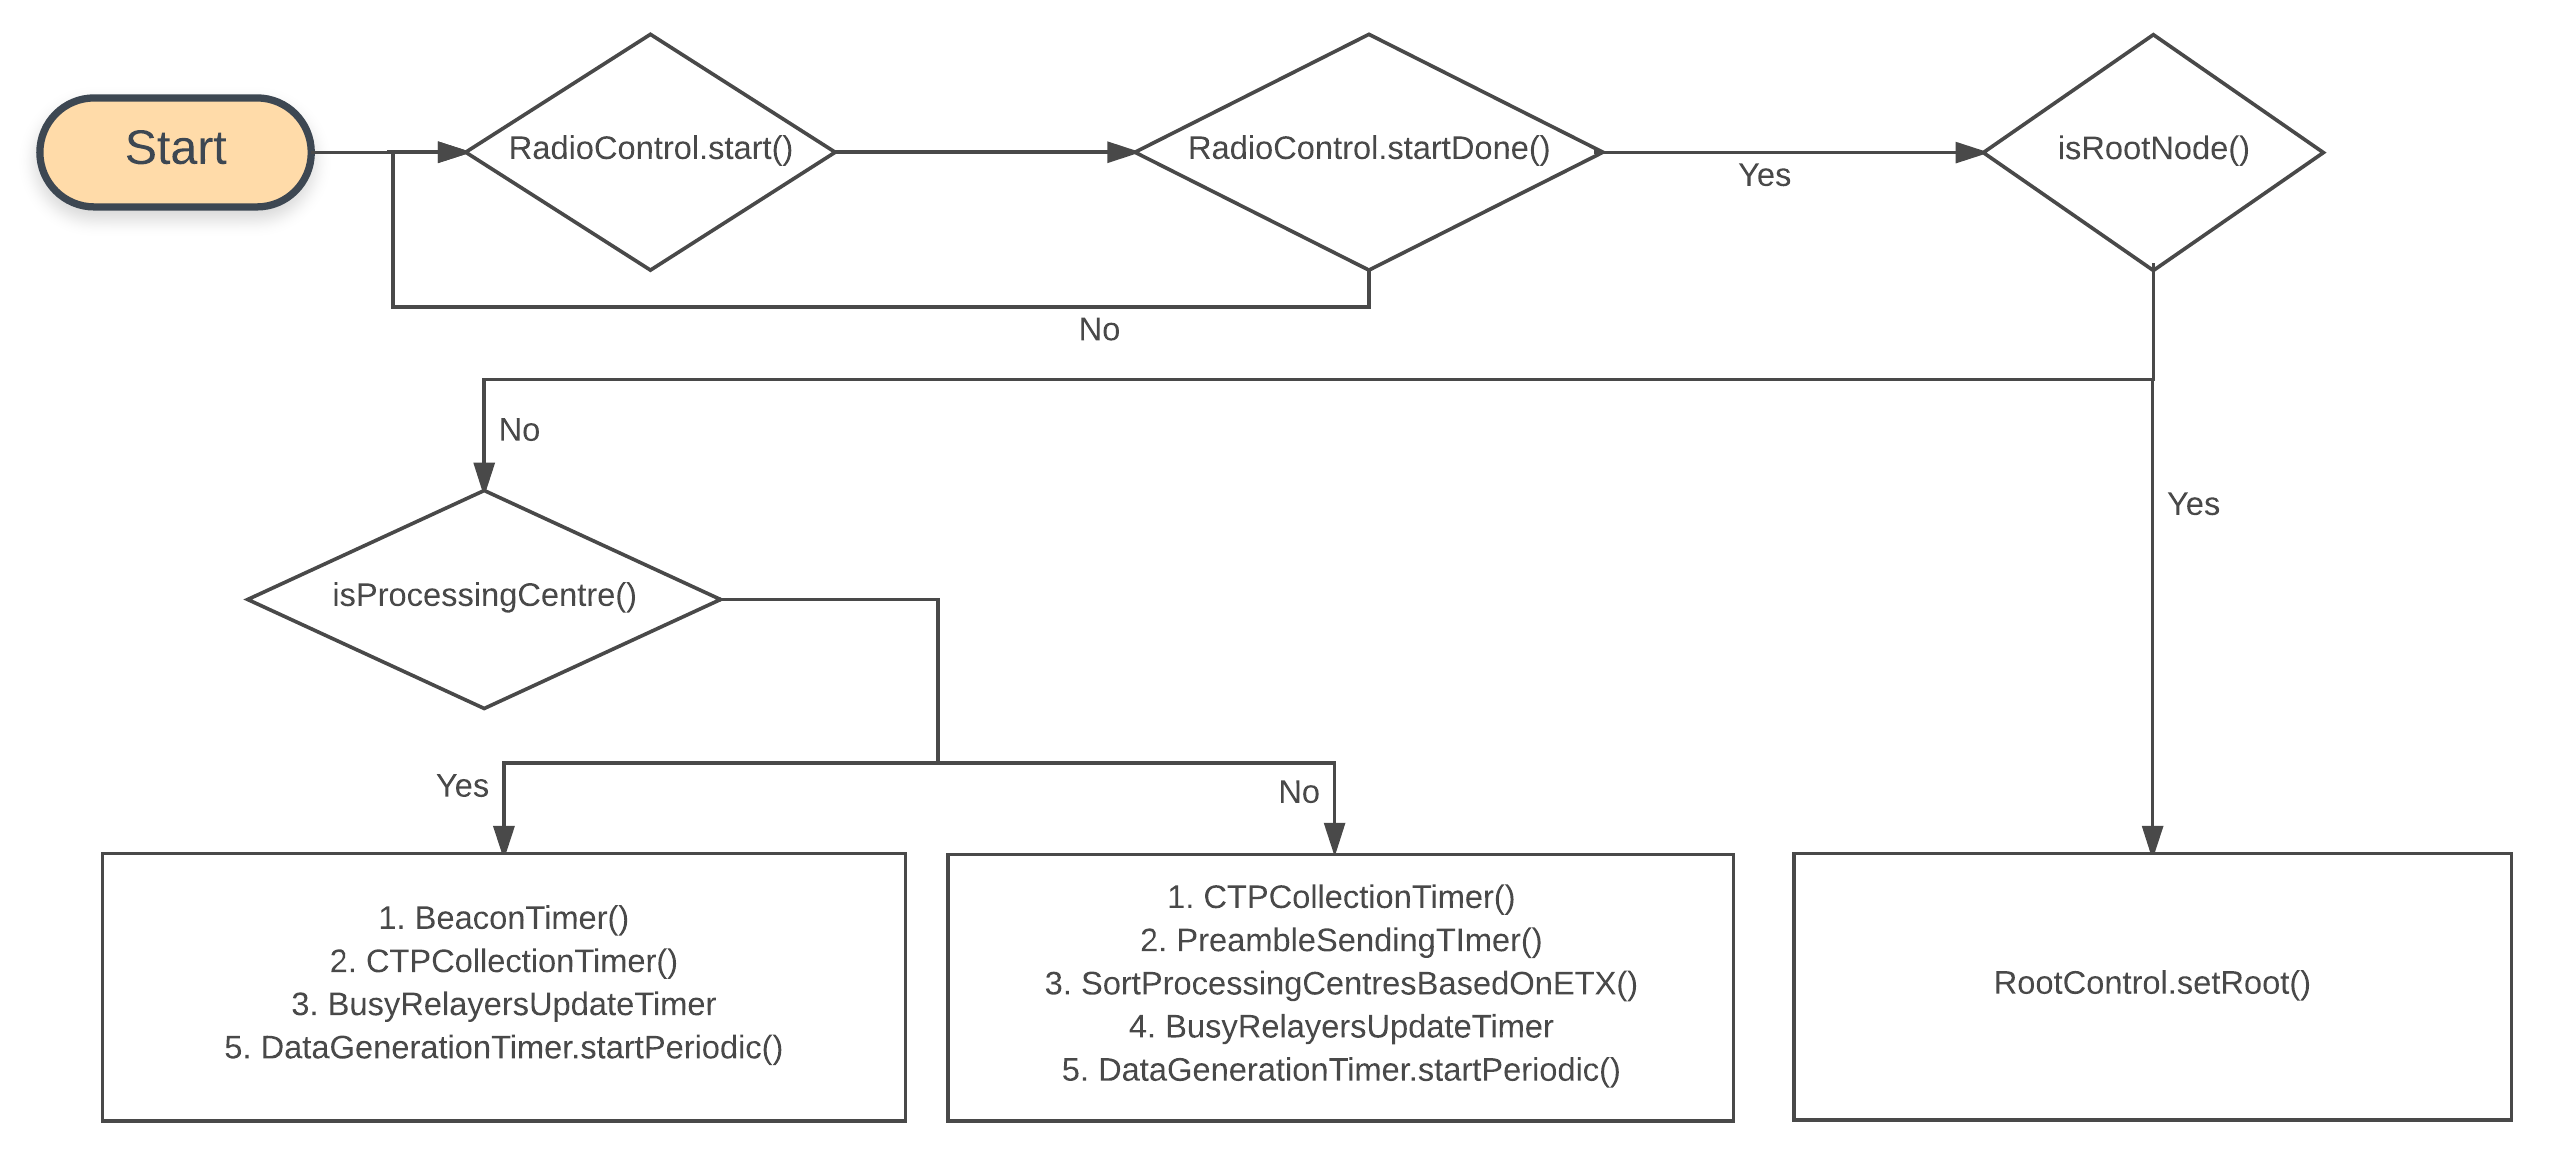
\includegraphics[width=1.0\textwidth]{gfx/Flow_diagram_start.png}
    \caption{Timer Interfaces in Heterogeneity}
    \label{fig:TimerInterfaces}
    \end{figure}

	
	In figure \ref{fig:TimerInterfaces}, we have illustrated a flow chart for the lifecycle of a \ac{SN} participating in heterogeneity design. Initially, every \ac{SN} turns it radio transceivers on and then, only when the RadioStart.startDone event signals without any errors, the \ac{SN} proceeds further to start certain timers. The selection of timers is based on two methods:
	
	\begin{enumerate}
	    \item isProcessingCentre: This method returns True, if the address of the current \ac{SN} (obtained by TOS\_NODE\_ID) matches a list of \acp{PC} defined as enum constants.
	    
	    \item isRootNode: This method returns True, if the address of the current \ac{SN} (obtained by TOS\_NODE\_ID) matches a list of \acp{BS} defined as enum constants.
	\end{enumerate}
	
	Based on the return values, appropriate timers are triggered. We will look at these timers in detail in coming subsections.
	    	
	%************************************************
	\subsection*{BeaconTimer}
	%************************************************
    
    It is a periodic timer fired by \ac{PC} at regular intervals. Figure \ref{fig:BeaconTimer} explains this concept in more detail. Firstly, each of the \acp{PC} checks sendBusyBeacon flag. If the flag is found not busy, a beacon, consisting of \ac{ETX} and \ac{PC}id, is broad-casted in one-hop neighborhood. On reception of these beacons, the \ac{SN} first update their local copy of processing centre struct array, which consists of \ac{PC} id, \ac{PC} \ac{ETX}, relayer id and relayer \ac{ETX} and then they forward it to their one hop neighbors. In the next subsection, we explain the PreambleSending Timer diagram which uses these updated local copy of \ac{PC} to send \ac{RTS} packets.

	\begin{figure}
    \centering
    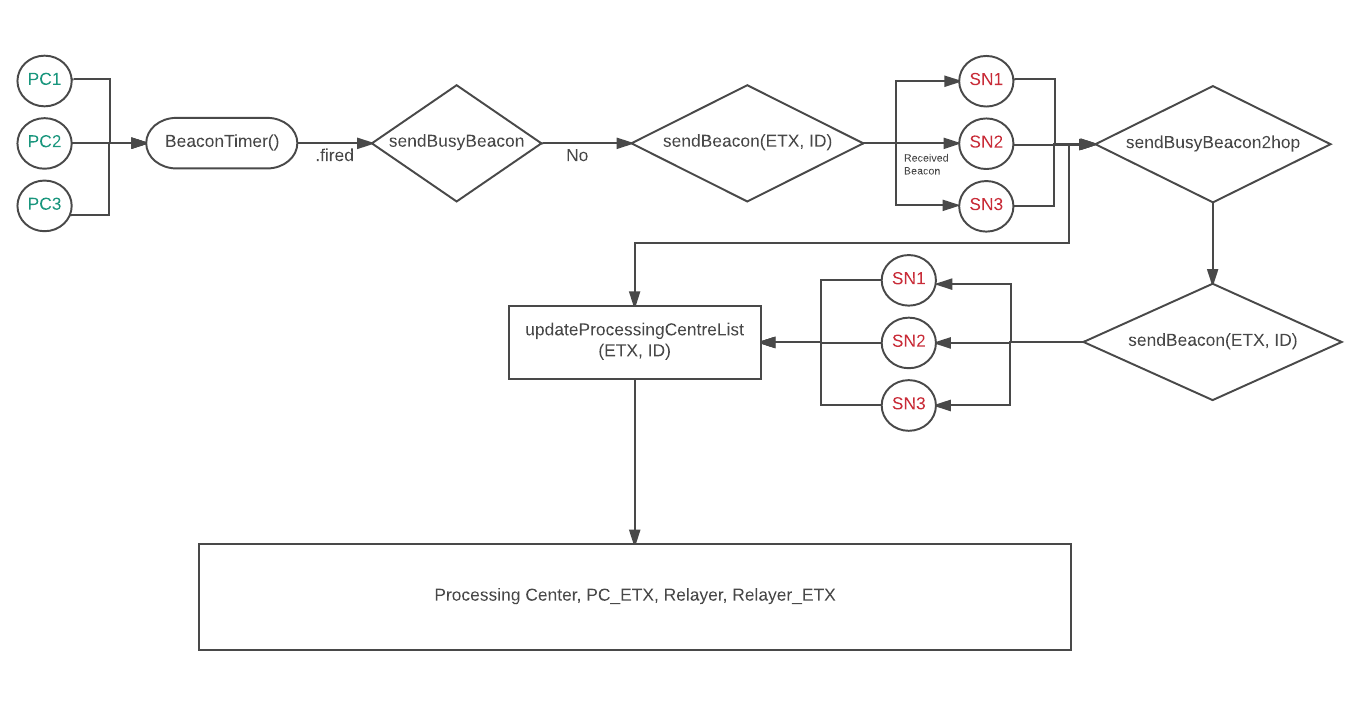
\includegraphics[width=1.0\textwidth]{gfx/BeaconTimer.png}
    \caption{Beacon Timer}
    \label{fig:BeaconTimer}
    \end{figure}
    
	%************************************************
	\subsection*{PreambleSendingTimer}
	%************************************************
	
	Each \ac{SN} maintains an updated list of \acp{PC} in two hop neighborhood and further sends a \ac{RTS} packet to request data processing by a \ac{PC}, based on the current state (occupied or free) of the \ac{SN}. We will explain this concept with the help of figure \ref{fig:PreambleTimer}. The model requires the sorted data from \textit{SortProcessingCentresBasedOnETX} timer. This timer periodically sorts the data in processing centre struct array based on lowest \ac{ETX} value and neighborhood distance. The PreambleSendingTimer then uses two arrays to decide whom to send \ac{RTS}: 1. sorted array of \acp{PC} and 2. busy \acp{PC} and relayers struct array (initially this list is empty, which means no \ac{PC} is busy initially). If a \ac{PC} is found by the method getProcessingCentreForTransmission using the above mentioned arrays, a \ac{RTS} packet is sent by setting transmitter address, receiver address, relayer address and duration of transfer desired as the packet contents. The recipient verifies if it is a relayer by extracting the relayer address from the packet contents (for a relayed transmission the packet content will have non-zero relayer address). In relayed transmission case, the packet is further forwarded to destination \ac{PC}. On reception of \ac{RTS} request by the \ac{PC}, it queues the request in CTSQueue and sends the \ac{CTS} response to the first \ac{RTS} sender. The sending response is broad-casted so that spectator \acp{SN} update their busy \acp{PC} and realyers struct array. This prevents other senders from not selecting an already occupied \ac{PC}. After getting the \ac{CTS} response, DataSendingTimer is fired which initiates the data transmission phase. The flowchart for DataSendingTimer is explained in next subsection.
	
	\begin{figure}
    \centering
    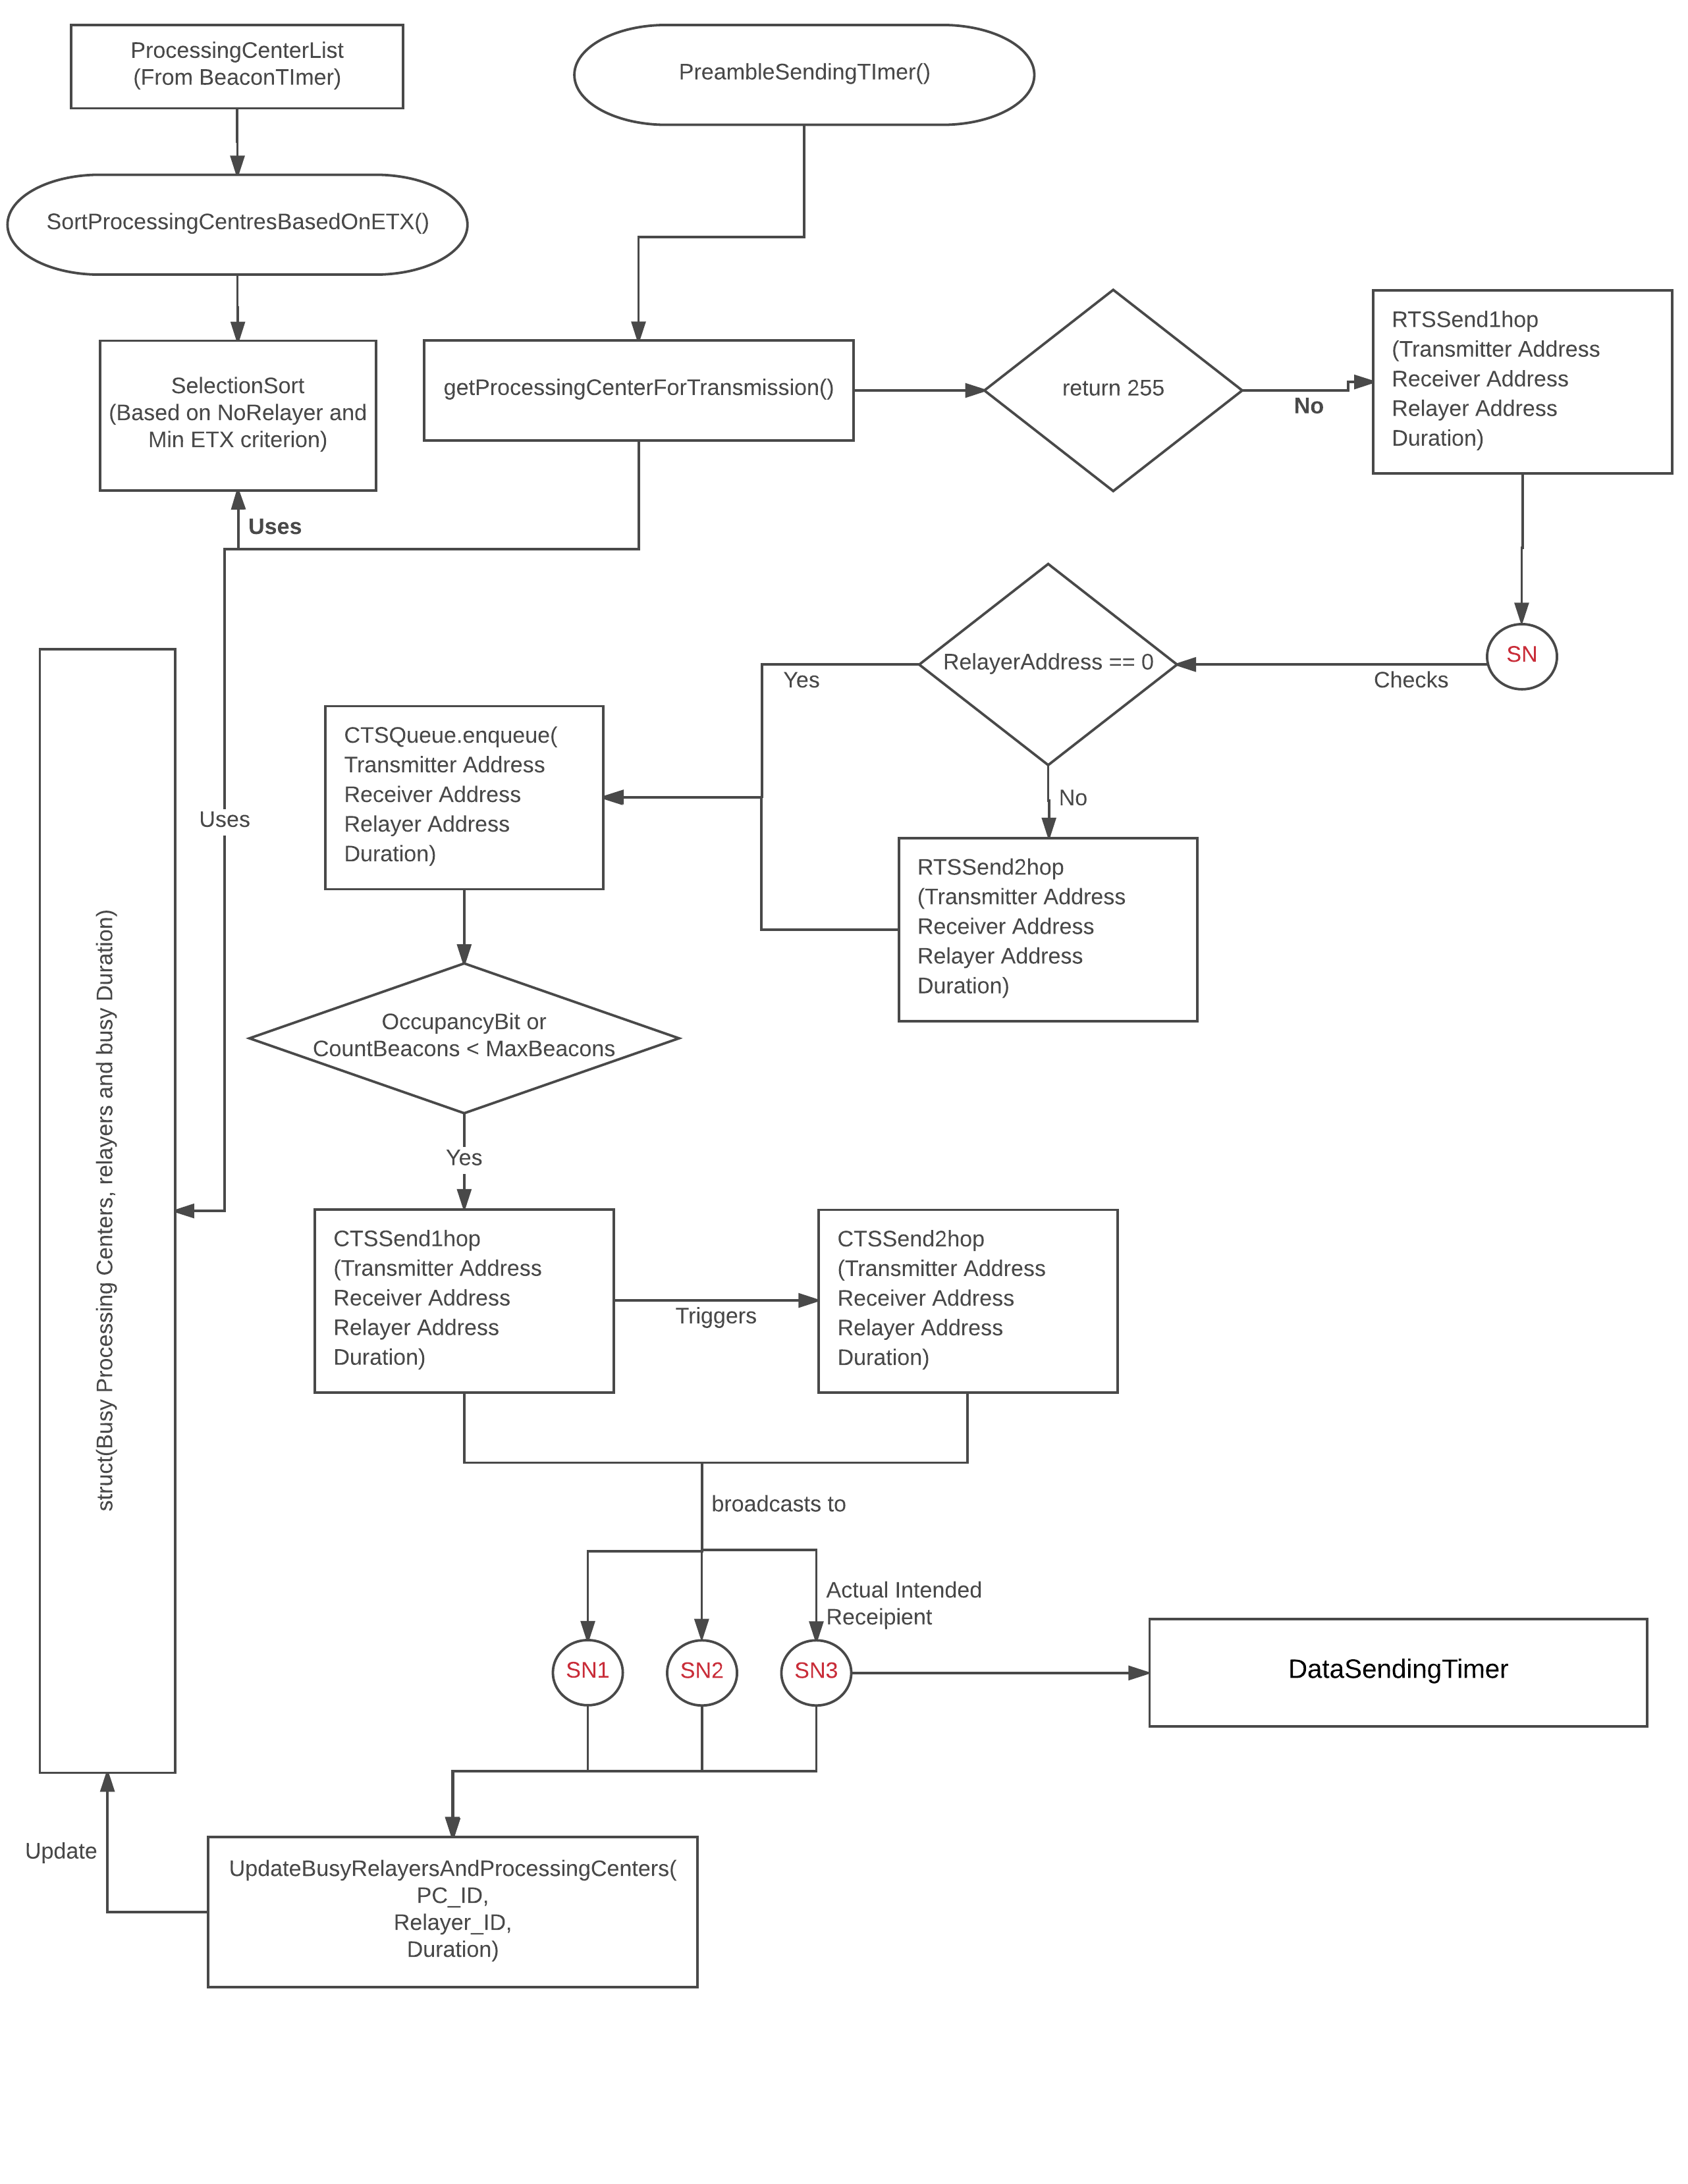
\includegraphics[width=1.0\textwidth]{gfx/PreambleSendingTimer.png}
    \caption{Beacon Timer}
    \label{fig:PreambleTimer}
    \end{figure}
    
	%************************************************
	\subsection*{DataSendingTimer}
	%************************************************
	
	DataSendingTimer is triggered only after \ac{RTS} response has been made by \ac{PC}. Figure \ref{fig:DataSendingTimer} elaborates the data sending concept of heterogeneity model in detail. Once data sending timer is fired, the intended sender verifies whether the time allotted to it is still remaining. If this condition holds, data is sent to the \ac{PC} or one hop relayer depending on whether it is one hop transmission or two hop transmission respectively. The AMSend.send signals send.sendDone event after successful or unsuccessful data transmission. We utilise this signalling event to again call data sending timer for sending the next packet. 
	
	\begin{figure}
    \centering
    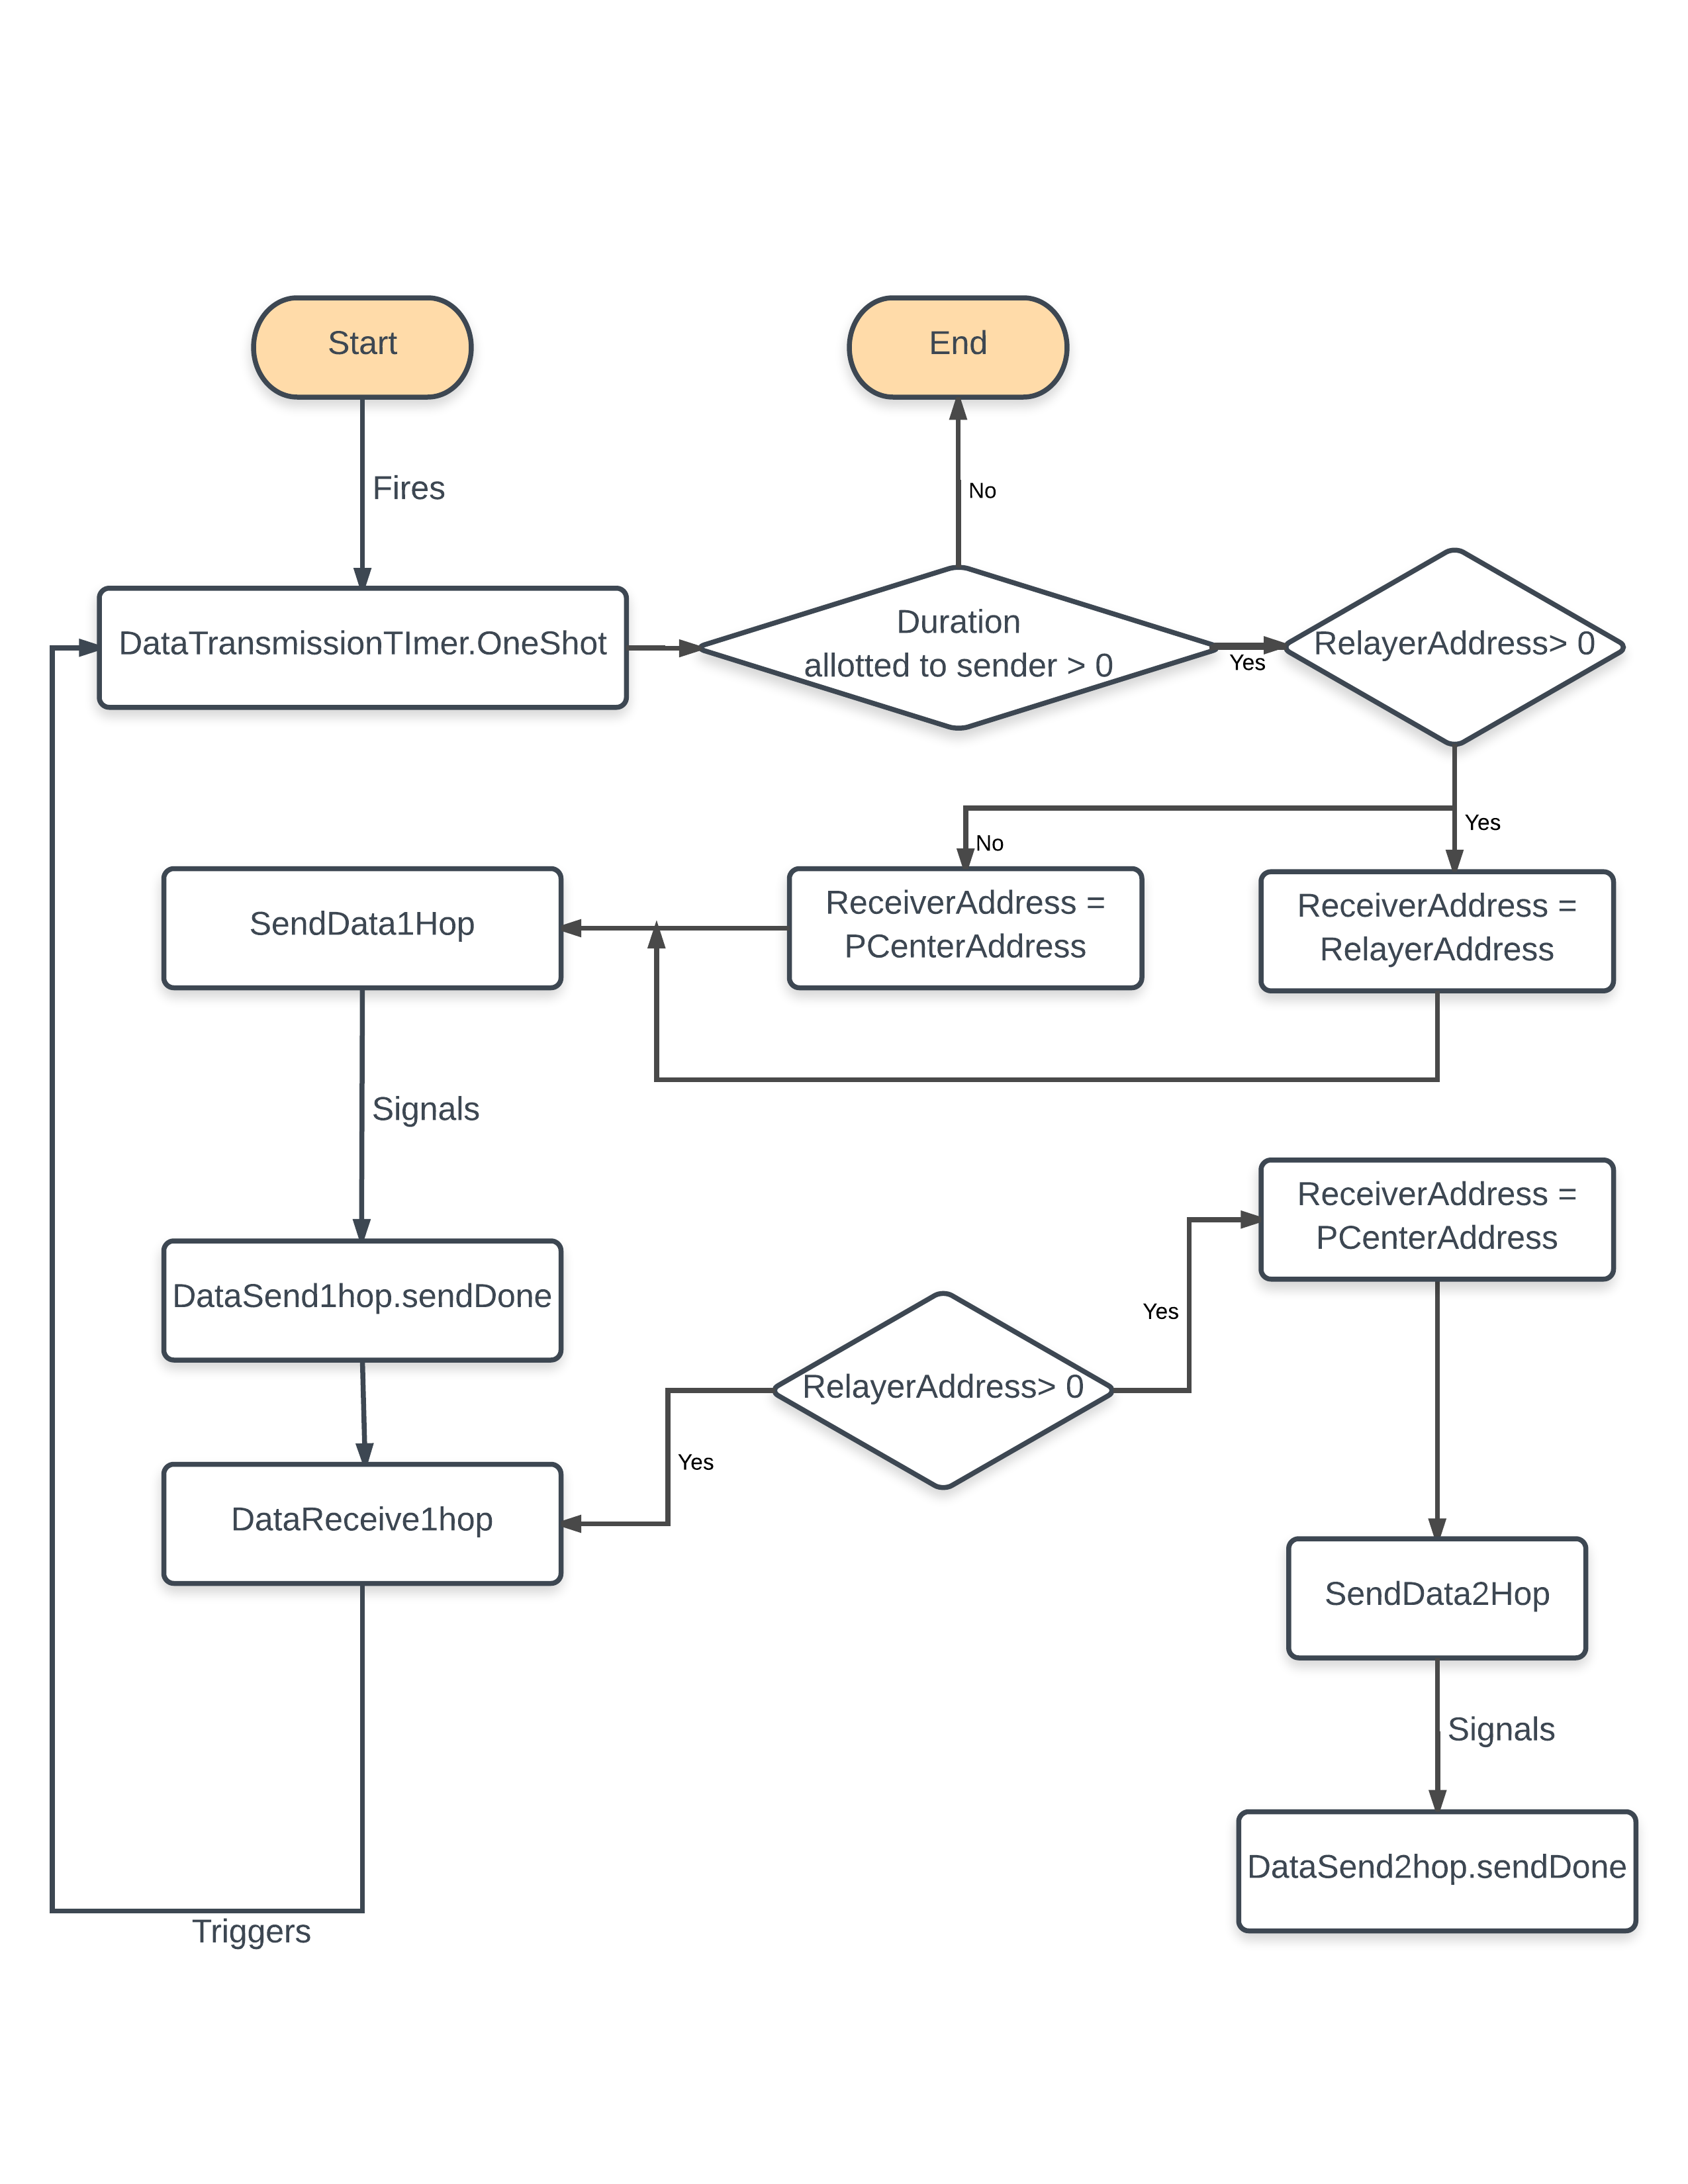
\includegraphics[width=1.0\textwidth]{gfx/DataSendingTimer.png}
    \caption{Data Sending Timer}
    \label{fig:DataSendingTimer}
    \end{figure}
    
        
	%************************************************
	\subsection*{CTPSendingTimer}
	%************************************************
	
	Data received by \ac{PC} is computed and added to CTPCollectionDataQueue. CTPTimer fires periodically and collects this data to route it via \ac{CTP} to \ac{BS}. If there are no elements in this queue, the timer uses DataGenerationQueue to route data via \ac{CTP}. DataGenerationQueue contains data acquired periodically by the \ac{SN}. For demonstrating heterogeneity, we have generated random numbers by periodically firing DataGenerationTimer. 
	This concept is shown in flowchart \ref{fig:CTPSendingTimer}.
    
    \begin{figure}
    \centering
    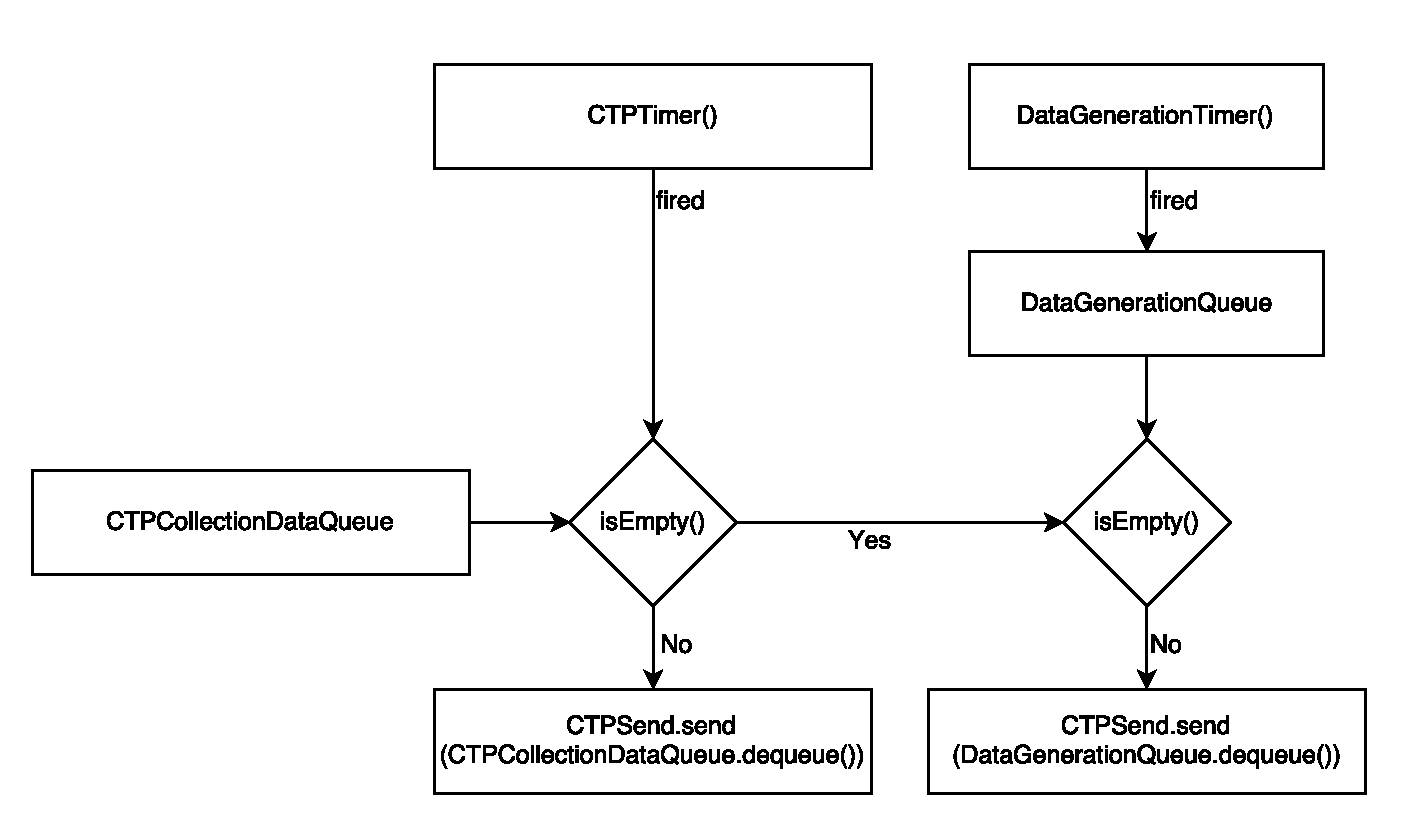
\includegraphics[width=1.0\textwidth]{gfx/CTPSendingTimer.pdf}
    \caption{\ac{CTP} Sending Timer}
    \label{fig:CTPSendingTimer}
    \end{figure}

% How the whole model looks as a process. What is the input and what is the output
% How the entire system looks like from a black box point of view.
% How do we regulate the concepts to make the ideas work?
% Keeping information upto date on timely basis
% Transition from the concept of timers to real time monitoring and checking of data transmission
    



% !TEX root = ../TUCthesis.tex

%************************************************
\chapter{Lots of lots of text}\label{ch:dummy}
%************************************************

\lipsum[1-30]

% !TEX root = ../TUCthesis.tex

%************************************************
\chapter{Conclusions/Discussions}\label{ch:conclusions}
%************************************************

The integration of wireless heterogeneous \acp{SN} in a \ac{WSN} is one of the most important features for future deployment of \ac{WSN}. In this project we have described the design and deployment of a wireless heterogeneous network on top of \acp{CTP}. We have used link estimation information from \acp{CTP} to make our network robust and thus adapt to the changes in the network. A policy-based mechanism has been deployed to monitor changes in the network, update the network with current state of neighbors and with minimal beacon usage, snoop the ongoing transmissions to make better decisions in occupying a free heterogeneous node. We have also compared performance, efficiency and reliability of the heterogeneity data transfer with the \acp{CTP} data transfer. From the experimental evaluations we have demonstrated significant advantages in placing a heterogeneous \acp{SN} in a \acp{WSN}. 

\par
We believe that with significant advancements in the network protocols and wireless sensor network devices in past decade, the focus of wireless sensor community will shift towards integration of heterogeneity in their protocols to make the network more energy efficient by providing data processing opportunity by a nearby \ac{SN}. This work has the potential to revolutionize the field of \acp{WSN}, by unifying heterogeneity with collection protocol and finally achieving highly enhanced data transmission capacity.


%************************************************
\section{Summary of Results}
%************************************************

Using heterogeneity layer over \ac{CTP} has demonstrated significant advantages experimentally. This is confirmed in the table \ref{tab:ProcessedvsUnprocessedData}. The data shows that we can send approximately seven times more data using heterogeneity to \ac{BS} than the \ac{CTP} layer at lower data transfer rates with around 91 percent reception and at higher data transfer rates we can send around three to four times more data to \acp{BS} with 95 percent packet reception. 

\begin{table}[h]
\caption{Number of data packets in CTP vs Heterogeneity} % title name of the table
\centering
\begin{adjustbox}{max width=\textwidth}

	\begin{tabular}{|c|c|c|} 
		\midrule
		Data Transfer Rate (in ms) & Packets received by heterogeneity (in thousands) & Packets received by \ac{CTP} (in thousands) \\
	    
	    50 & 50.89 & 7.21 \\
	    80 & 36.66 & 7.32 \\
	    100 & 28.18 & 7.60 \\
	    120 & 23.88 & 7.55 \\
	    150 & 18.98 & 7.60 \\
	    180 & 16.97 & 7.60 \\
	    200 & 15.11 & 7.62 \\
	    220 & 13.19 & 7.66 \\
	    230 & 12.90 & 7.64 \\
	    250 & 13.12 & 7.77 \\
		\hline
		\end{tabular}
\end{adjustbox} 	
\label{tab:ProcessedvsUnprocessedData}
\end{table}


%************************************************
\section{Recommendations for Further Research}
%************************************************

It can be seen from the table \ref{tab:PRRinHeterogeneity} that we are not able to increase \acp{PRR} beyond 96 percent. This motivates us to carry out more experiments to see how heterogeneity works in conjunction with other collection protocols. 
    
\begin{table}[h]
\caption{PRR} % title name of the table
\centering
\begin{adjustbox}{max width=\textwidth}

	\begin{tabular}{|c|c|} 
		\midrule
		Data Transfer Rate (in ms) & \ac{PRR} (in percentage) \\
	    50 & 91.9 \\
	    80 & 92.3 \\
	    100 & 94.4 \\
	    120 & 94.8 \\
	    150 & 94.8 \\
	    180 & 95.6 \\
	    200 & 95.2 \\
	    220 & 95.6 \\
	    230 & 94.8 \\
	    250 & 95.3 \\
		\hline
		\end{tabular}
\end{adjustbox} 	
\label{tab:PRRinHeterogeneity}
\end{table}

This research work has also opened up a large number of topics for further research. Since, we have experimentally verified the concept of heterogeneity using \acp{CTP}, therefore now we need to examine the compatibility of heterogeneity with other network protocols. We also believe that the heterogeneity layer needs to be more generalised to accommodate diversity of application scenarios. From the algorithmic point of view, this protocol needs refinement in terms of allowing more than two hop neighborhood search area and also provide flexibility in selecting a \acp{PC} not only based on the measure of \acp{ETX} values but also other useful \acp{LQI}. 

\par
Further, we need to mitigate causes for not achieving 100 percent data delivery. Therefore, we need to study the efficiency of retransmission cache in heterogeneity to achieve 100 percent packet reception. We can further work towards reducing the number of beacon exchanges and work out an efficient way to encode more information with minimal beacon exchanges. 

\par
We further need to examine the possibility of integrating other major design features suggested by other researchers in our protocol. For example, the paper \cite{zhao2004energy} provides an algorithm to find out the optimal cluster heads in a \ac{WSN} without involving the \ac{BS}. We can integrate this in our algorithm to find out which of the nodes in the network are the most suitable contestants for being a \acp{PC}. 

% \begin{enumerate}
    
%     \item Design improvements: To let users choose how many hop they want to deep dig to find the processing center
    
% \end{enumerate}


% \begin{enumerate}
%     \item 
    
%     Can also wait for a while and let the queue fill up to select the CTS request which fits the best among all. So instead of responding to the CTS request the \ac{PC} can wait for a while and respond to the optimum option
    
%     More generalisation in terms of interfaces and make it as an extensible parameter to other classes
    
%     Optimal code so that the process does not have to o through loops multiple times. Instead store with some kind of mapping tables. 
    
    
%     \item Algorithm improvements: Now there is only a possibility to choose the best neighbour based on ETX. later we can add support for multiple sorting choices like best etx, random chosing, backtracking old data before choosing one like how many times CTS request was rejected.
    
    
%     Adaptive beaconing to adapt to data changes
    
%     Tweak parameters to test how the system reacts to changing RREQ or RTS and RREP or CTS mechanism and do not doing them at all.
    
%     The sequence number of data packets can help track the lost packets and in certain  scenarios it can be beneficial to track which packets are lost in the course of data transmission. This can further avoid transient routing loops of exponentially flooded packets incase retransmit cache is calle dto send the lost packets. Looping packets must have a modified sequence number say a packet with sequence number 12 can be retarnsmitted again with sequence number 12.1 to keep the receiving nodes aware that this is the first copy of the lost packet.
    
%     another possibility to reduce loss is to remove the sensor node participating in heterogenity from \ac{ctp}
    
%     see how sending after 2hop data transmission has completed 
    
%     reduce the number of beacon exchanges for heterogeneity model
    
%     see how the hetergeneity layer behaves with other collection protocols. Given that we replace \ac{ETX} metric with the metric used in the chosen collection protocol
        
% \end{enumerate}

%%********************************************************************
%% Other Stuff in the Back
%%*******************************************************
\cleardoublepage
\printbibliography[heading=classicthesis]

%% Uncomment following lines if an appendix is needed
\appendix\cleardoublepage
% !TEX root = ../TUCthesis.tex 

%********************************************************************
% Appendix
%*******************************************************
% If problems with the headers: get headings in appendix etc. right
%\markboth{\spacedlowsmallcaps{Appendix}}{\spacedlowsmallcaps{Appendix}}
\chapter{Appendix Test}
Lorem ipsum at nusquam appellantur his, ut eos erant homero
concludaturque. Albucius appellantur deterruisset id eam, vivendum
partiendo dissentiet ei ius. Vis melius facilisis ea, sea id convenire
referrentur, takimata adolescens ex duo. Ei harum argumentum per. Eam
vidit exerci appetere ad, ut vel zzril intellegam interpretaris.

Errem omnium ea per, pro congue populo ornatus cu, ex qui dicant
nemore melius. No pri diam iriure euismod. Graecis eleifend
appellantur quo id. Id corpora inimicus nam, facer nonummy ne pro,
kasd repudiandae ei mei. Mea menandri mediocrem dissentiet cu, ex
nominati imperdiet nec, sea odio duis vocent ei. Tempor everti
appareat cu ius, ridens audiam an qui, aliquid admodum conceptam ne
qui. Vis ea melius nostrum, mel alienum euripidis eu.

\section{Appendix Section Test}
Test: \autoref{tab:moreexample} (This reference should have a 
lowercase, small caps \spacedlowsmallcaps{A} if the option 
\texttt{floatperchapter} is activated, just as in the table itself
 $\rightarrow$ however, this does not work at the moment.)

\begin{table}[h]
    \myfloatalign
  \begin{tabularx}{\textwidth}{Xll} \toprule
    \tableheadline{labitur bonorum pri no} & \tableheadline{que vista}
    & \tableheadline{human} \\ \midrule
    fastidii ea ius & germano &  demonstratea \\
    suscipit instructior & titulo & personas \\
    %postulant quo & westeuropee & sanctificatec \\
    \midrule
    quaestio philosophia & facto & demonstrated \\
    %autem vulputate ex & parola & romanic \\
    %usu mucius iisque & studio & sanctificatef \\
    \bottomrule
  \end{tabularx}
  \caption[Autem usu id]{Autem usu id.}
  \label{tab:moreexample}
\end{table}

%Nulla fastidii ea ius, exerci suscipit instructior te nam, in ullum
%postulant quo. Congue quaestio philosophia his at, sea odio autem
%vulputate ex. Cu usu mucius iisque voluptua. Sit maiorum propriae at,
%ea cum primis intellegat. Hinc cotidieque reprehendunt eu nec. Autem
%timeam deleniti usu id, in nec nibh altera.




\section{Another Appendix Section Test}
Equidem detraxit cu nam, vix eu delenit periculis. Eos ut vero
constituto, no vidit propriae complectitur sea. Diceret nonummy in
has, no qui eligendi recteque consetetur. Mel eu dictas suscipiantur,
et sed placerat oporteat. At ipsum electram mei, ad aeque atomorum
mea. There is also a useless Pascal listing below: \autoref{lst:useless}.

\begin{lstlisting}[float=b,language=Pascal,frame=tb,caption={A floating example (\texttt{listings} manual)},label=lst:useless]
for i:=maxint downto 0 do
begin
{ do nothing }
end;
\end{lstlisting}

%Ei solet nemore consectetuer nam. Ad eam porro impetus, te choro omnes
%evertitur mel. Molestie conclusionemque vel at, no qui omittam
%expetenda efficiendi. Eu quo nobis offendit, verterem scriptorem ne
%vix.



%% ********************************************************************
%% Game Over: Restore, Restart, or Quit?
%%*******************************************************
\end{document}
%% ********************************************************************
